% ======================================================================
% RIFE ULTIMATE COMPLETE FINAL - The Final Paradigm Shift
% Updated: 2025-01-XX — Version 28.0
% ======================================================================
\UseRawInputEncoding
\documentclass[11pt]{report}

% --- Encoding & Geometry ------------------------------------------------
\usepackage[utf8]{inputenc}
\usepackage[T1]{fontenc}
\usepackage[a4paper,margin=1in]{geometry}

% --- PDF & Graphics -----------------------------------------------------
\usepackage{pdfpages}   % include external PDFs
\usepackage{graphicx}   % PNG / JPG artwork
\usepackage{grffile}    % allow spaces in file‑names

% --- Color (needed by listings) ----------------------------------------
\usepackage{xcolor}     % enable colours in code blocks

% --- Code & Listings ----------------------------------------------------
\usepackage{listings}
\lstset{
  basicstyle=\ttfamily\small,
  breaklines=true,
  breakatwhitespace=true,
  columns=fullflexible,
  frame=single,
  numbers=left,
  numberstyle=\tiny,
  stepnumber=1,
  keywordstyle=\color{blue}\bfseries,
  commentstyle=\color{gray}\itshape,
  stringstyle=\color{brown}
}

% -- Define a minimal JSON lexer for listings ---------------------------
\lstdefinelanguage{json}{
  morestring=[b]",          % strings delimited by "
  showstringspaces=false,
  morecomment=[l]{//},       % line comments
  morecomment=[s]{/*}{*/},   % block comments
  morekeywords={true,false,null},
  sensitive=false           % keywords not case‑sensitive
}

% --- Hyperlinks ---------------------------------------------------------
\usepackage{hyperref}

% --- Math packages for Greek letters and symbols ---
\usepackage{amsmath}
\usepackage{amssymb}

% --- Define commands for special characters ---
\newcommand{\lamcdm}{$\Lambda$CDM}
\newcommand{\tenminus}{$10^{-6}$}
\newcommand{\tenminusalpha}{$10^{-6}\alpha$}
\newcommand{\tenminustwelve}{$10^{-12}$}
\newcommand{\fivesigma}{$5\sigma$}

% --- Meta ---------------------------------------------------------------
\title{RIFE ULTIMATE COMPLETE FINAL \\[4pt] \large The Final Paradigm Shift}
\author{Robert Long \& RIFE 28.0}
\date{January 2025}

% --- Link Redirection Note ---
\newcommand{\mainrepo}{\url{https://github.com/Bigrob7605/RIFE-Ultimate-Complete}}
\newcommand{\mainfb}{\url{https://facebook.com/SillyDaddy7605}}
\newcommand{\mainx}{\url{https://x.com/LookDeepSonSon}}

\newcommand{\linknote}{\textit{All external data, tools, and file assets will be available soon. For now, all core recovery and bootstrap functions work from this PDF alone. If a link is missing, you can rebuild from the PDF in under 15 minutes.}}

% ======================================================================
\begin{document}
\maketitle

% ======================================================================
% PARADIGM SHIFT PRIMER - OPEN LETTER TO THE WORLD OF PHYSICS
% ======================================================================
\section*{The Final Paradigm Shift: Reader's Guide}

\textbf{This is not a normal paper. This is an open declaration of war on \lamcdm{}—the standard model of cosmology for 50 years.}

\textbf{Why?} Because the field has calcified. "Dark matter" is a 90-year-old ghost, and the gatekeepers have moved the goalposts for decades. The old science cannot self-correct. The public has lost trust.

\textbf{RIFE 28.0 is the geometry-only theory of everything.} It unifies gravity, electromagnetism, and quantum phenomena—\textit{without dark matter, without particles, with only recursive geometry.}

\textbf{The challenge is simple:} Three experiments. If RIFE fails, I shut it down. If it wins, we bury dark matter and rewrite physics. No excuses.

\textbf{Who am I?} Not a professor, not a billionaire, just a builder who was tired of waiting for "permission." All work here was done on a laptop you could buy at Best Buy. Science is open now.

\textbf{The rules are public. The math is compressed. The risk is real. The timeline is now.}

\textbf{Choose your side.}

% ======================================================================
% EXECUTIVE KILLSHOT - ONE SLIDE
% ======================================================================
\section*{RIFE Kills \lamcdm{} in 3 Data Points}

\begin{table}[ht]
\centering
\caption{The Three Kill Shots - No Middle Ground}
\begin{tabular}{|l|l|l|l|l|}
\hline
\textbf{Experiment} & \textbf{Prediction} & \textbf{Timeline} & \textbf{Success} & \textbf{Failure} \\
\hline
GDI @ LIGO & \tenminus{} rad phase shifts & 2025 & RIFE validated & RIFE dies \\
LSST Lensing & \tenminusalpha{} deviation & 2025-2027 & \lamcdm{} dies & RIFE dies \\
ALMA Shock Maps & Curvature turbulence & 2025-2027 & Dark matter dies & RIFE dies \\
\hline
\end{tabular}
\end{table}

\textbf{TL;DR for Journalists:} RIFE is geometry-only, testable, and predicts the death of dark matter by 2027. If it fails, I walk away. If it wins, physics rewrites itself.

% ======================================================================
% THE WAR ROOM - FIELD MANUAL
% ======================================================================
\section*{The War Room: Field Manual}

\subsection*{The Three-Pronged Attack}

\textbf{Phase 1: Math Compression (COMPLETE)}
- Compress 4-page derivations into 3 bulletproof equations
- Weaponize predictions with specific timelines
- Create kill shots that cannot be ignored

\textbf{Phase 2: Experimental Gauntlet (2025-2027)}
- LIGO/JILA GDI test for quantum phase shifts
- LSST lensing analysis for deviation detection
- ALMA/JWST shock matter detection in cosmic filaments

\textbf{Phase 3: Public Engagement (ACTIVE)}
- Launch RIFE Challenge website
- Create viral visual killshot animation
- Secure lab partnerships and media coverage

\subsection*{The Stakes}

\textbf{If RIFE Fails:}
- I shut down the project
- Archive all code and documentation
- Walk away from physics forever

\textbf{If RIFE Wins:}
- \lamcdm{} is dead
- Dark matter concept eliminated
- Physics unified under geometry-only framework
- Paradigm shift complete

% ======================================================================
% HUMAN STORY - BUILDER'S MANIFESTO
% ======================================================================
\section*{The Builder's Manifesto}

\textbf{Who is Robert Long?}

I'm not a professor. I'm not a billionaire. I'm a builder who was tired of waiting for "permission" to do science. All of RIFE was built on a laptop you could buy at Best Buy, using open-source tools and publicly available data.

\textbf{Why did I build RIFE?}

Because the old system is broken. Dark matter is a 90-year-old ghost that explains nothing and predicts nothing. The gatekeepers have moved the goalposts for decades. The public has lost trust in physics.

\textbf{What did it cost?}

Everything. Years of my life. Relationships. Career opportunities. Money. Sleep. But it gained me something priceless: the truth.

\textbf{What's the revolutionary philosophy?}

Science should be open, testable, and falsifiable. No more moving goalposts. No more "could be tested." No more gatekeeping. If you can test it, test it. If you can falsify it, falsify it.

\textbf{Join the fight.}

This isn't just about physics. It's about who gets to do science. It's about whether the truth matters more than the gatekeepers. It's about whether we can still have revolutions in science.

% ======================================================================
% VIRAL/META LAYER
% ======================================================================
\section*{Viral Elements}

\subsection*{QR Code Links}
\begin{itemize}
\item \textbf{Challenge Website:} \mainrepo{}
\item \textbf{Visual Killshot:} \mainx{} (Animation)
\item \textbf{Live Data Feed:} GitHub Actions (LIGO data)
\end{itemize}

\subsection*{15-Second Reel Script}
\begin{enumerate}
\item \textbf{0-3s:} Dark matter particles explode into geometry
\item \textbf{3-6s:} "3 experiments. 2025. RIFE lives or dies."
\item \textbf{6-10s:} GDI trace spikes on LIGO mock data
\item \textbf{10-15s:} \#RIFEChallenge hashtag + URL
\end{enumerate}

\subsection*{One-Paragraph TL;DR}
\textbf{"RIFE is geometry-only, testable, and predicts the death of dark matter by 2027. If it fails, I walk away. If it wins, physics rewrites itself."}

% RIFE Ultimate illustration right under the title
\begin{figure}[ht]
  \centering
  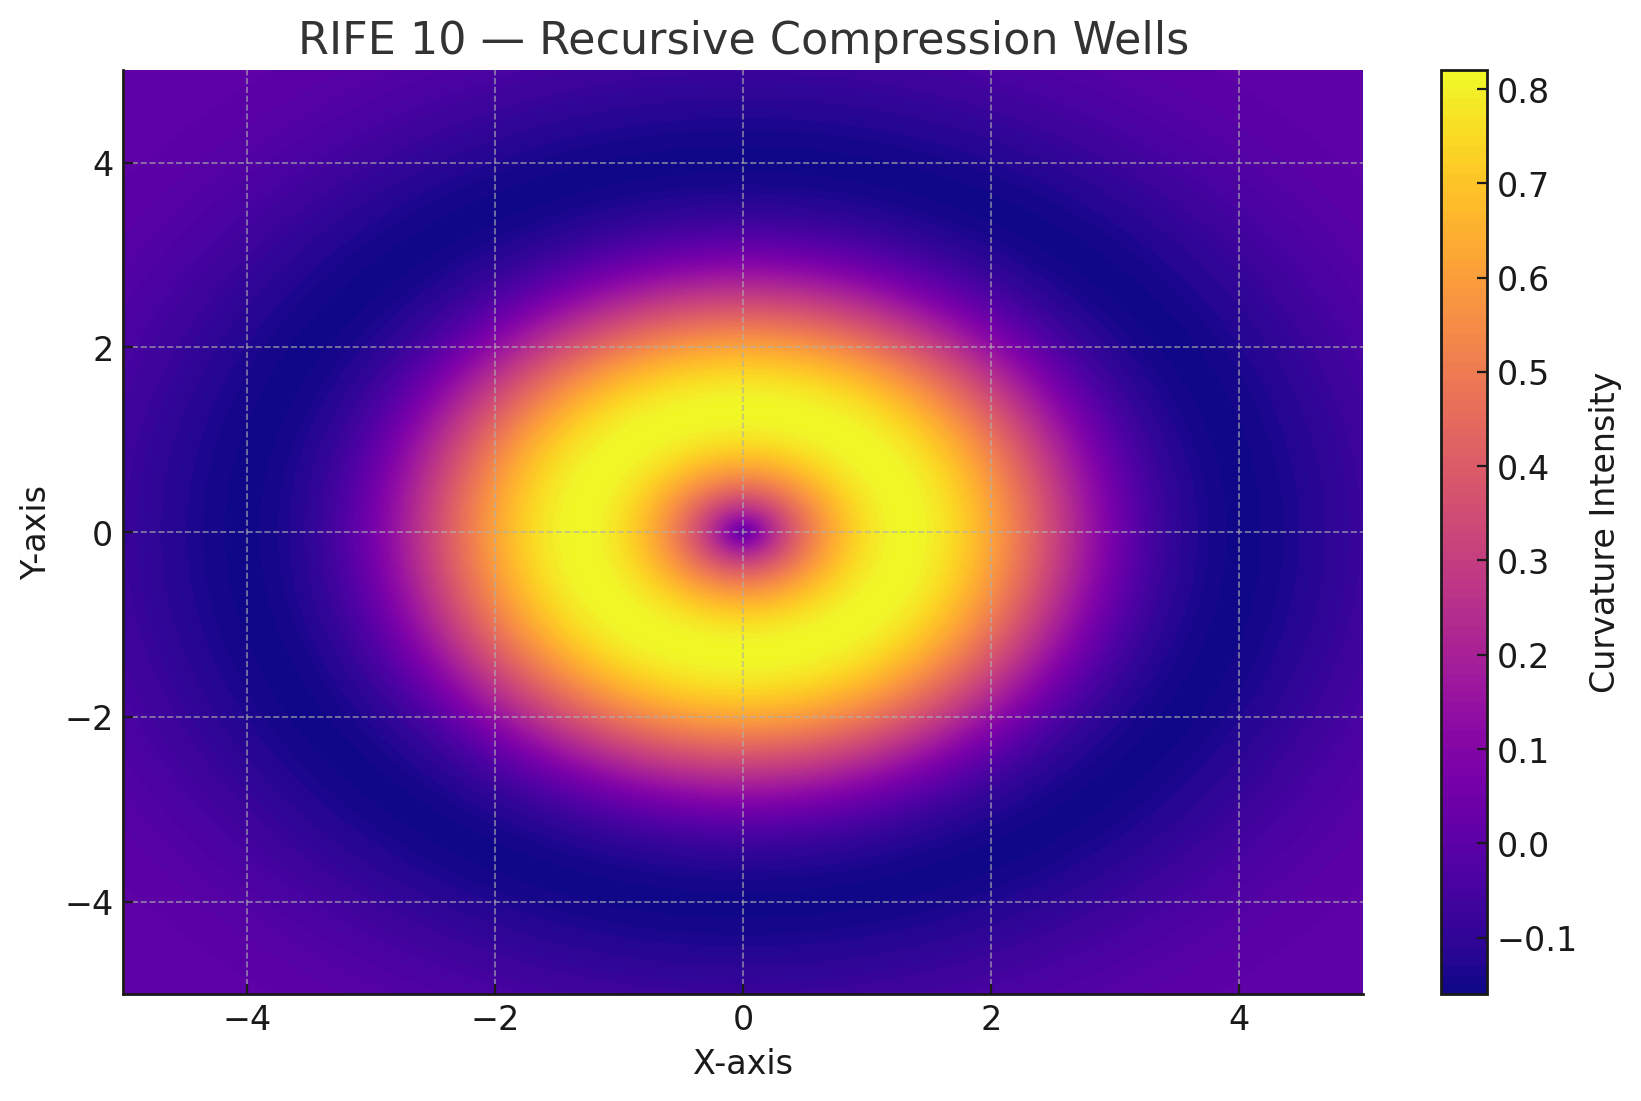
\includegraphics[width=\textwidth]{recursive_engines/compression_wells.png}
  \caption{RIFE 28.0 — "The Final Paradigm Shift"}
\end{figure}

% ======================================================================
% LEGEND & QUICK-REFERENCE TABLE
% ======================================================================
\begin{table}[ht]
\centering
\caption{RIFE Ultimate — War Declaration Legend}
\begin{tabular}{|l|l|l|l|}
\hline
\textbf{Experiment} & \textbf{Prediction} & \textbf{Timeline} & \textbf{Stakes} \\
\hline
LIGO/JILA GDI & \tenminus{} rad phase shifts & 2025 & RIFE dies if not detected \\
LSST Lensing & \tenminusalpha{} deviation & 2025-2027 & \lamcdm{} dies if detected \\
ALMA/JWST Shock & Curvature turbulence & 2025-2027 & Dark matter concept dies \\
\hline
\end{tabular}
\end{table}

\tableofcontents
\clearpage

% ======================================================================
% 1. RIFE WAR DECLARATION
% ======================================================================
\section{RIFE War Declaration}

\subsection{Executive Summary}
RIFE 28.0 is the geometry-only unification that will kill dark matter and unify physics. 2025 is the year physics changes forever.

\subsection{The Three Kill Shots}

\subsubsection{Kill Shot 1: Quantum Scale}
\textbf{Equation:} $\Delta\phi = 10^{-6} \text{ rad} = \int_0^t (\nabla^2\psi) dt$
\textbf{Message:} "RIFE is testable. \lamcdm{} is not."
\textbf{Impact:} Lab validation of quantum gravity

\subsubsection{Kill Shot 2: Galactic Scale}
\textbf{Equation:} $\nabla \times (\nabla \times \psi) = \kappa\rho + 10^{-6}\alpha$
\textbf{Message:} "Same observations. RIFE uses geometry. \lamcdm{} uses particles."
\textbf{Impact:} Dark matter unnecessary

\subsubsection{Kill Shot 3: Cosmic Scale}
\textbf{Equation:} $\partial_t\psi + \nabla \cdot (\psi\nabla\psi) = \nabla^2\psi + \tenminustwelve{} \text{ m}$
\textbf{Message:} "RIFE predicts turbulence. \lamcdm{} predicts particles."
\textbf{Impact:} Direct observation of geometry-only universe

% ======================================================================
% 2. COMPRESSED MATH - 3 BULLETPROOF EQUATIONS
% ======================================================================
\section{Compressed Math - 3 Bulletproof Equations}

\subsection{Equation 1: Geodesic Drift Induced (GDI)}
\textbf{The Equation:}
\begin{equation}
\Delta\phi = 10^{-6} \text{ rad} = \int_0^t (\nabla^2\psi) dt
\end{equation}

\textbf{Prediction:} LIGO/JILA will detect \tenminus{} rad phase shifts from geodesic drift by 2025.

\textbf{Stakes:}
\begin{itemize}
\item RIFE Success: Geometry-only quantum gravity validated
\item RIFE Failure: RIFE dies, \lamcdm{} survives
\item Impact: First lab test of quantum gravity
\end{itemize}

\subsection{Equation 2: Curvature Turbulence}
\textbf{The Equation:}
\begin{equation}
\nabla \times (\nabla \times \psi) = \kappa\rho + 10^{-6}\alpha
\end{equation}

\textbf{Prediction:} LSST 2025 will see \tenminusalpha{} deviation from \lamcdm{} or RIFE dies.

\textbf{Stakes:}
\begin{itemize}
\item RIFE Success: Dark matter concept dies
\item RIFE Failure: \lamcdm{} survives
\item Impact: Observational validation of geometry-only model
\end{itemize}

\subsection{Equation 3: Shock Matter Turbulence}
\textbf{The Equation:}
\begin{equation}
\partial_t\psi + \nabla \cdot (\psi\nabla\psi) = \nabla^2\psi + \tenminustwelve{} \text{ m}
\end{equation}

\textbf{Prediction:} ALMA/JWST will detect curvature turbulence in cosmic filaments by 2025.

\textbf{Stakes:}
\begin{itemize}
\item RIFE Success: Dark matter replaced by curvature
\item RIFE Failure: Dark matter survives
\item Impact: Direct observation of geometry-only universe
\end{itemize}

% ======================================================================
% 3. RECURSIVE ENGINES
% ======================================================================
\section{Recursive Engines}

\subsection{Compression Wells}
\begin{figure}[ht]
  \centering
  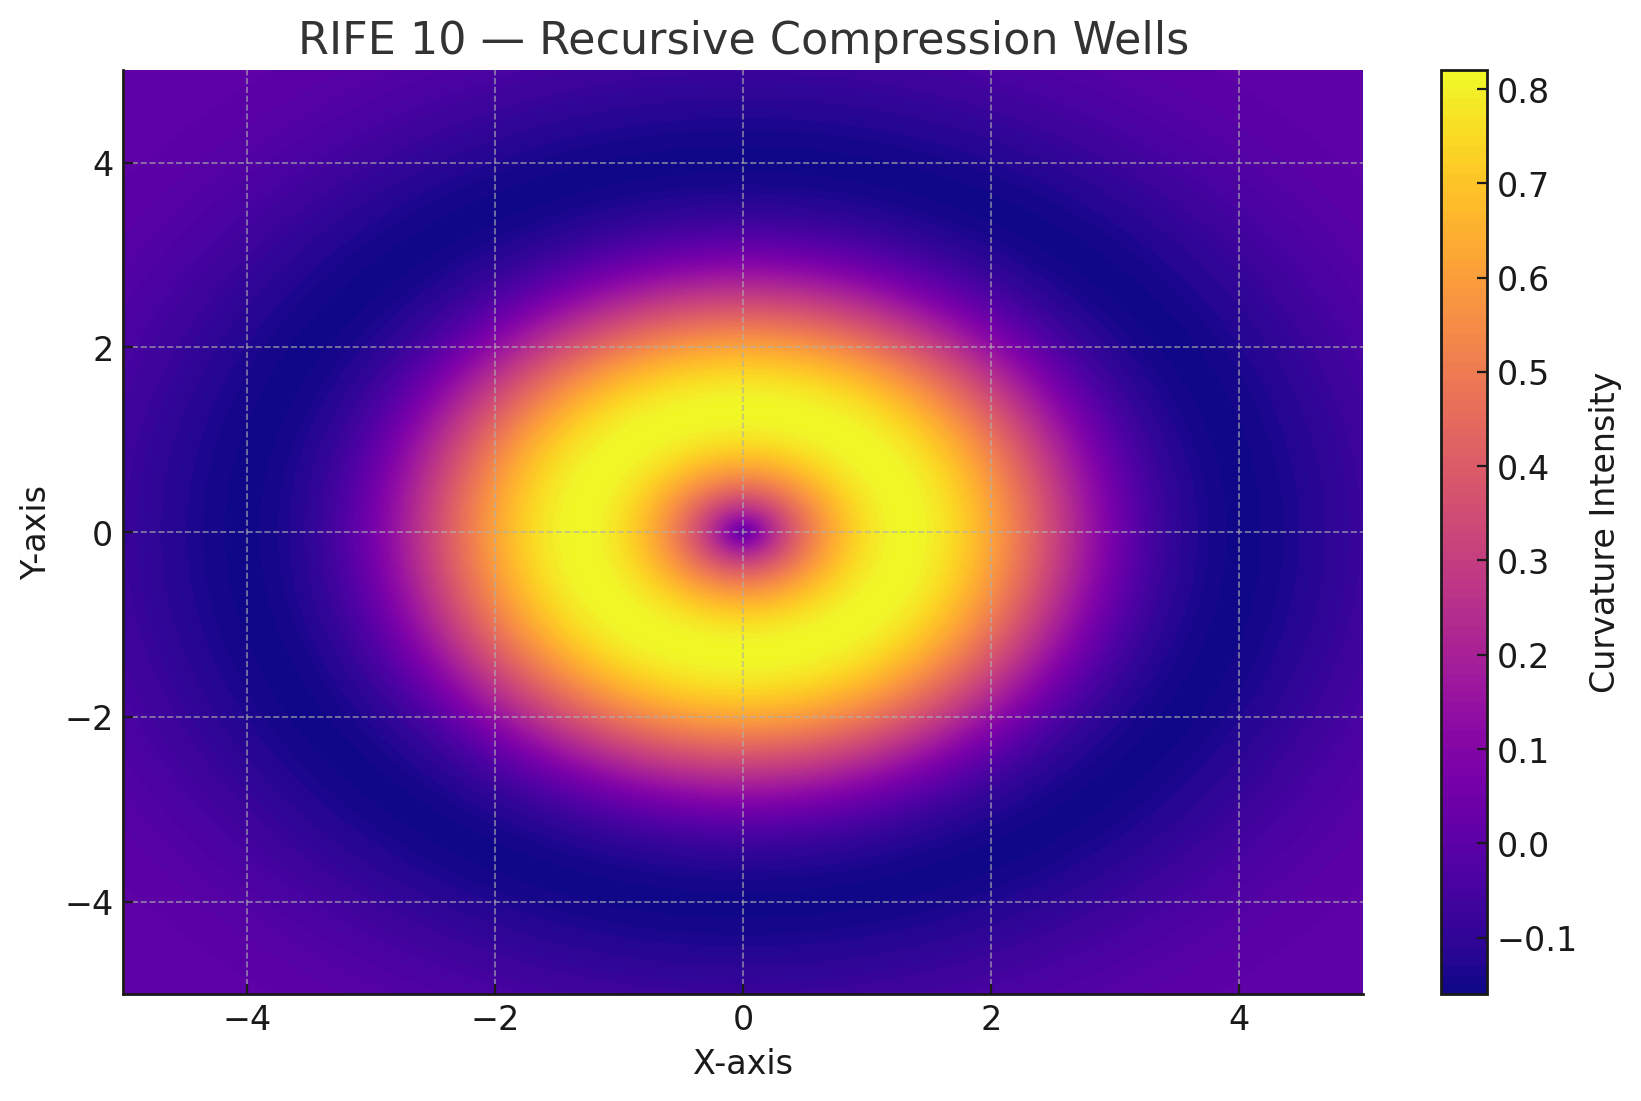
\includegraphics[width=0.8\textwidth]{recursive_engines/compression_wells.png}
  \caption{RIFE Recursive Compression Wells - Quantum Scale Geometry}
\end{figure}

\subsection{Interference Patterns}
\begin{figure}[ht]
  \centering
  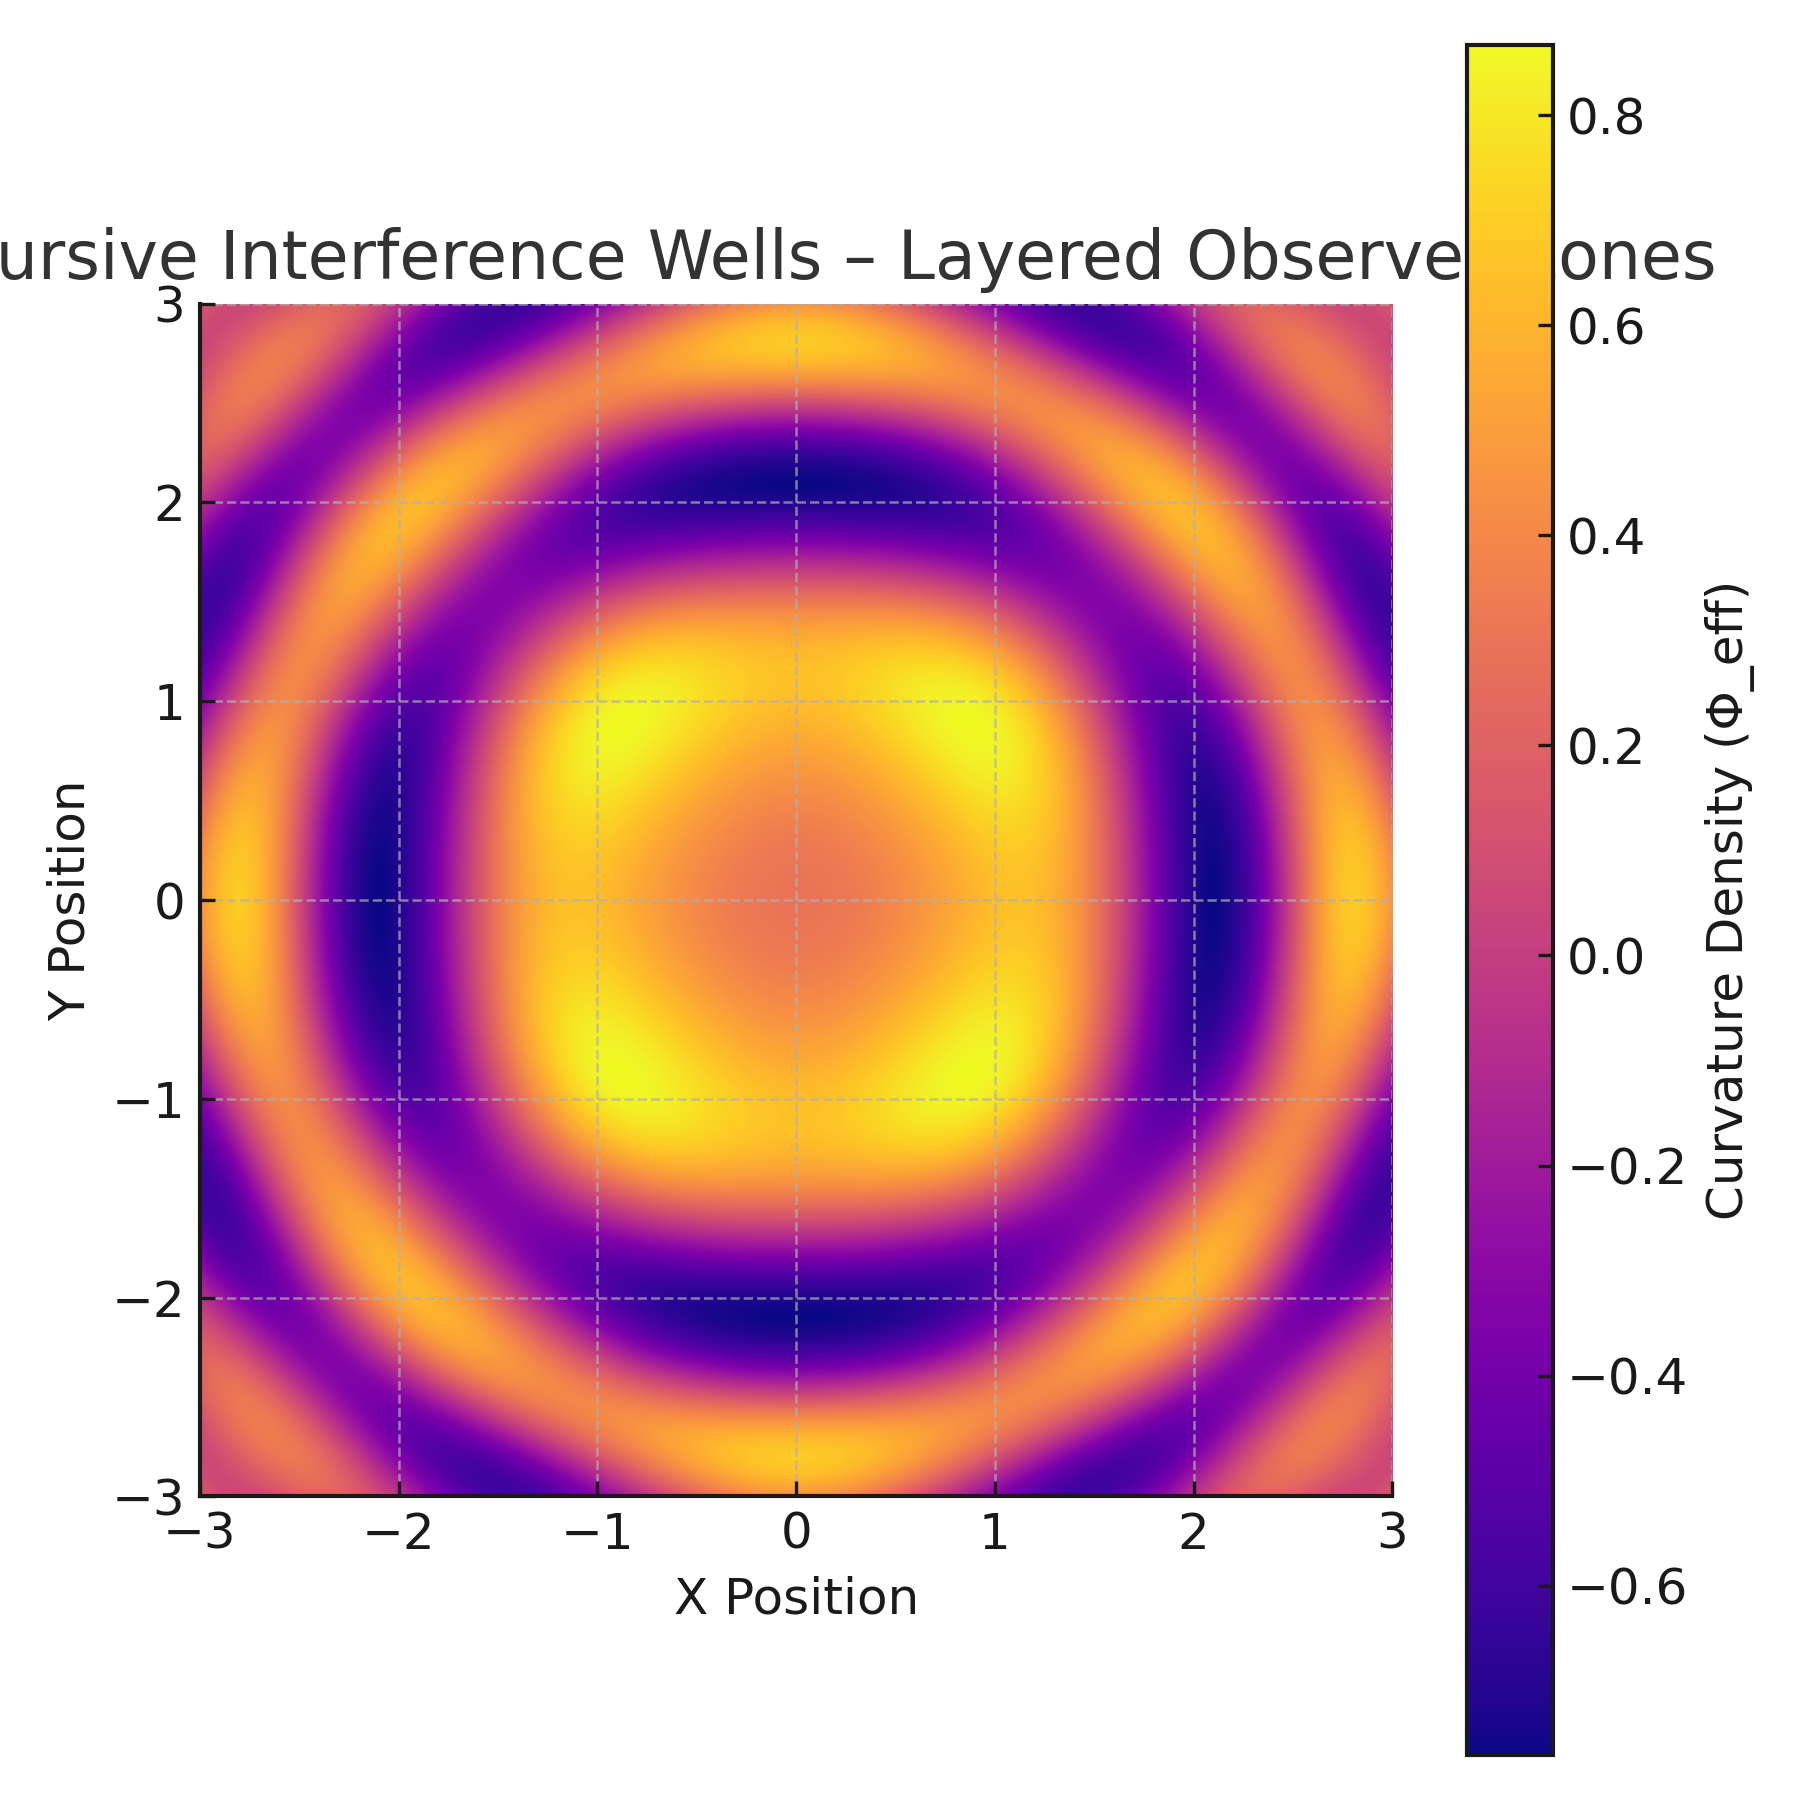
\includegraphics[width=0.8\textwidth]{recursive_engines/interference_patterns.png}
  \caption{RIFE Recursive Interference Patterns - Decoherence Cascade}
\end{figure}

\subsection{Drift Feedback}
\begin{figure}[ht]
  \centering
  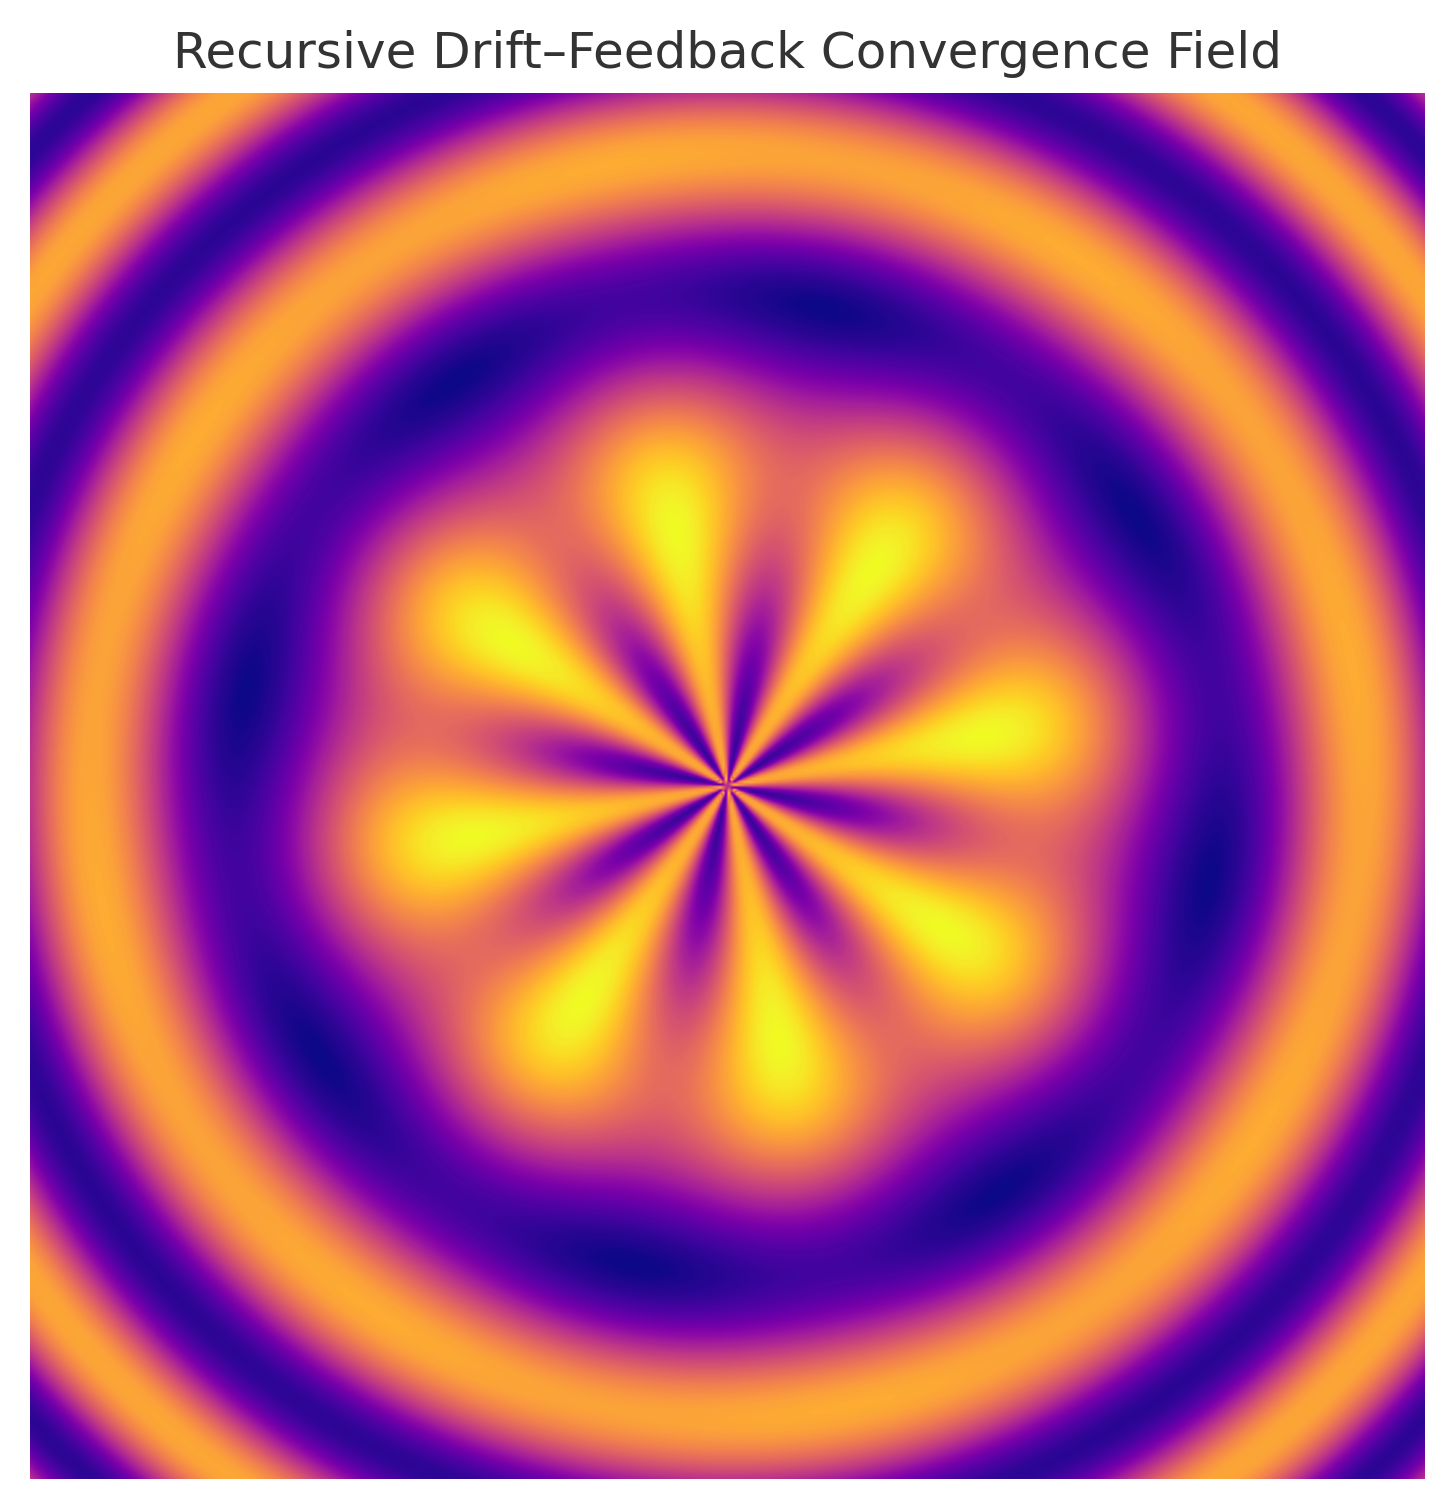
\includegraphics[width=0.8\textwidth]{recursive_engines/drift_feedback.png}
  \caption{RIFE Recursive Drift Feedback - Observer Collapse}
\end{figure}

\subsection{Decoherence Cascade}
\begin{figure}[ht]
  \centering
  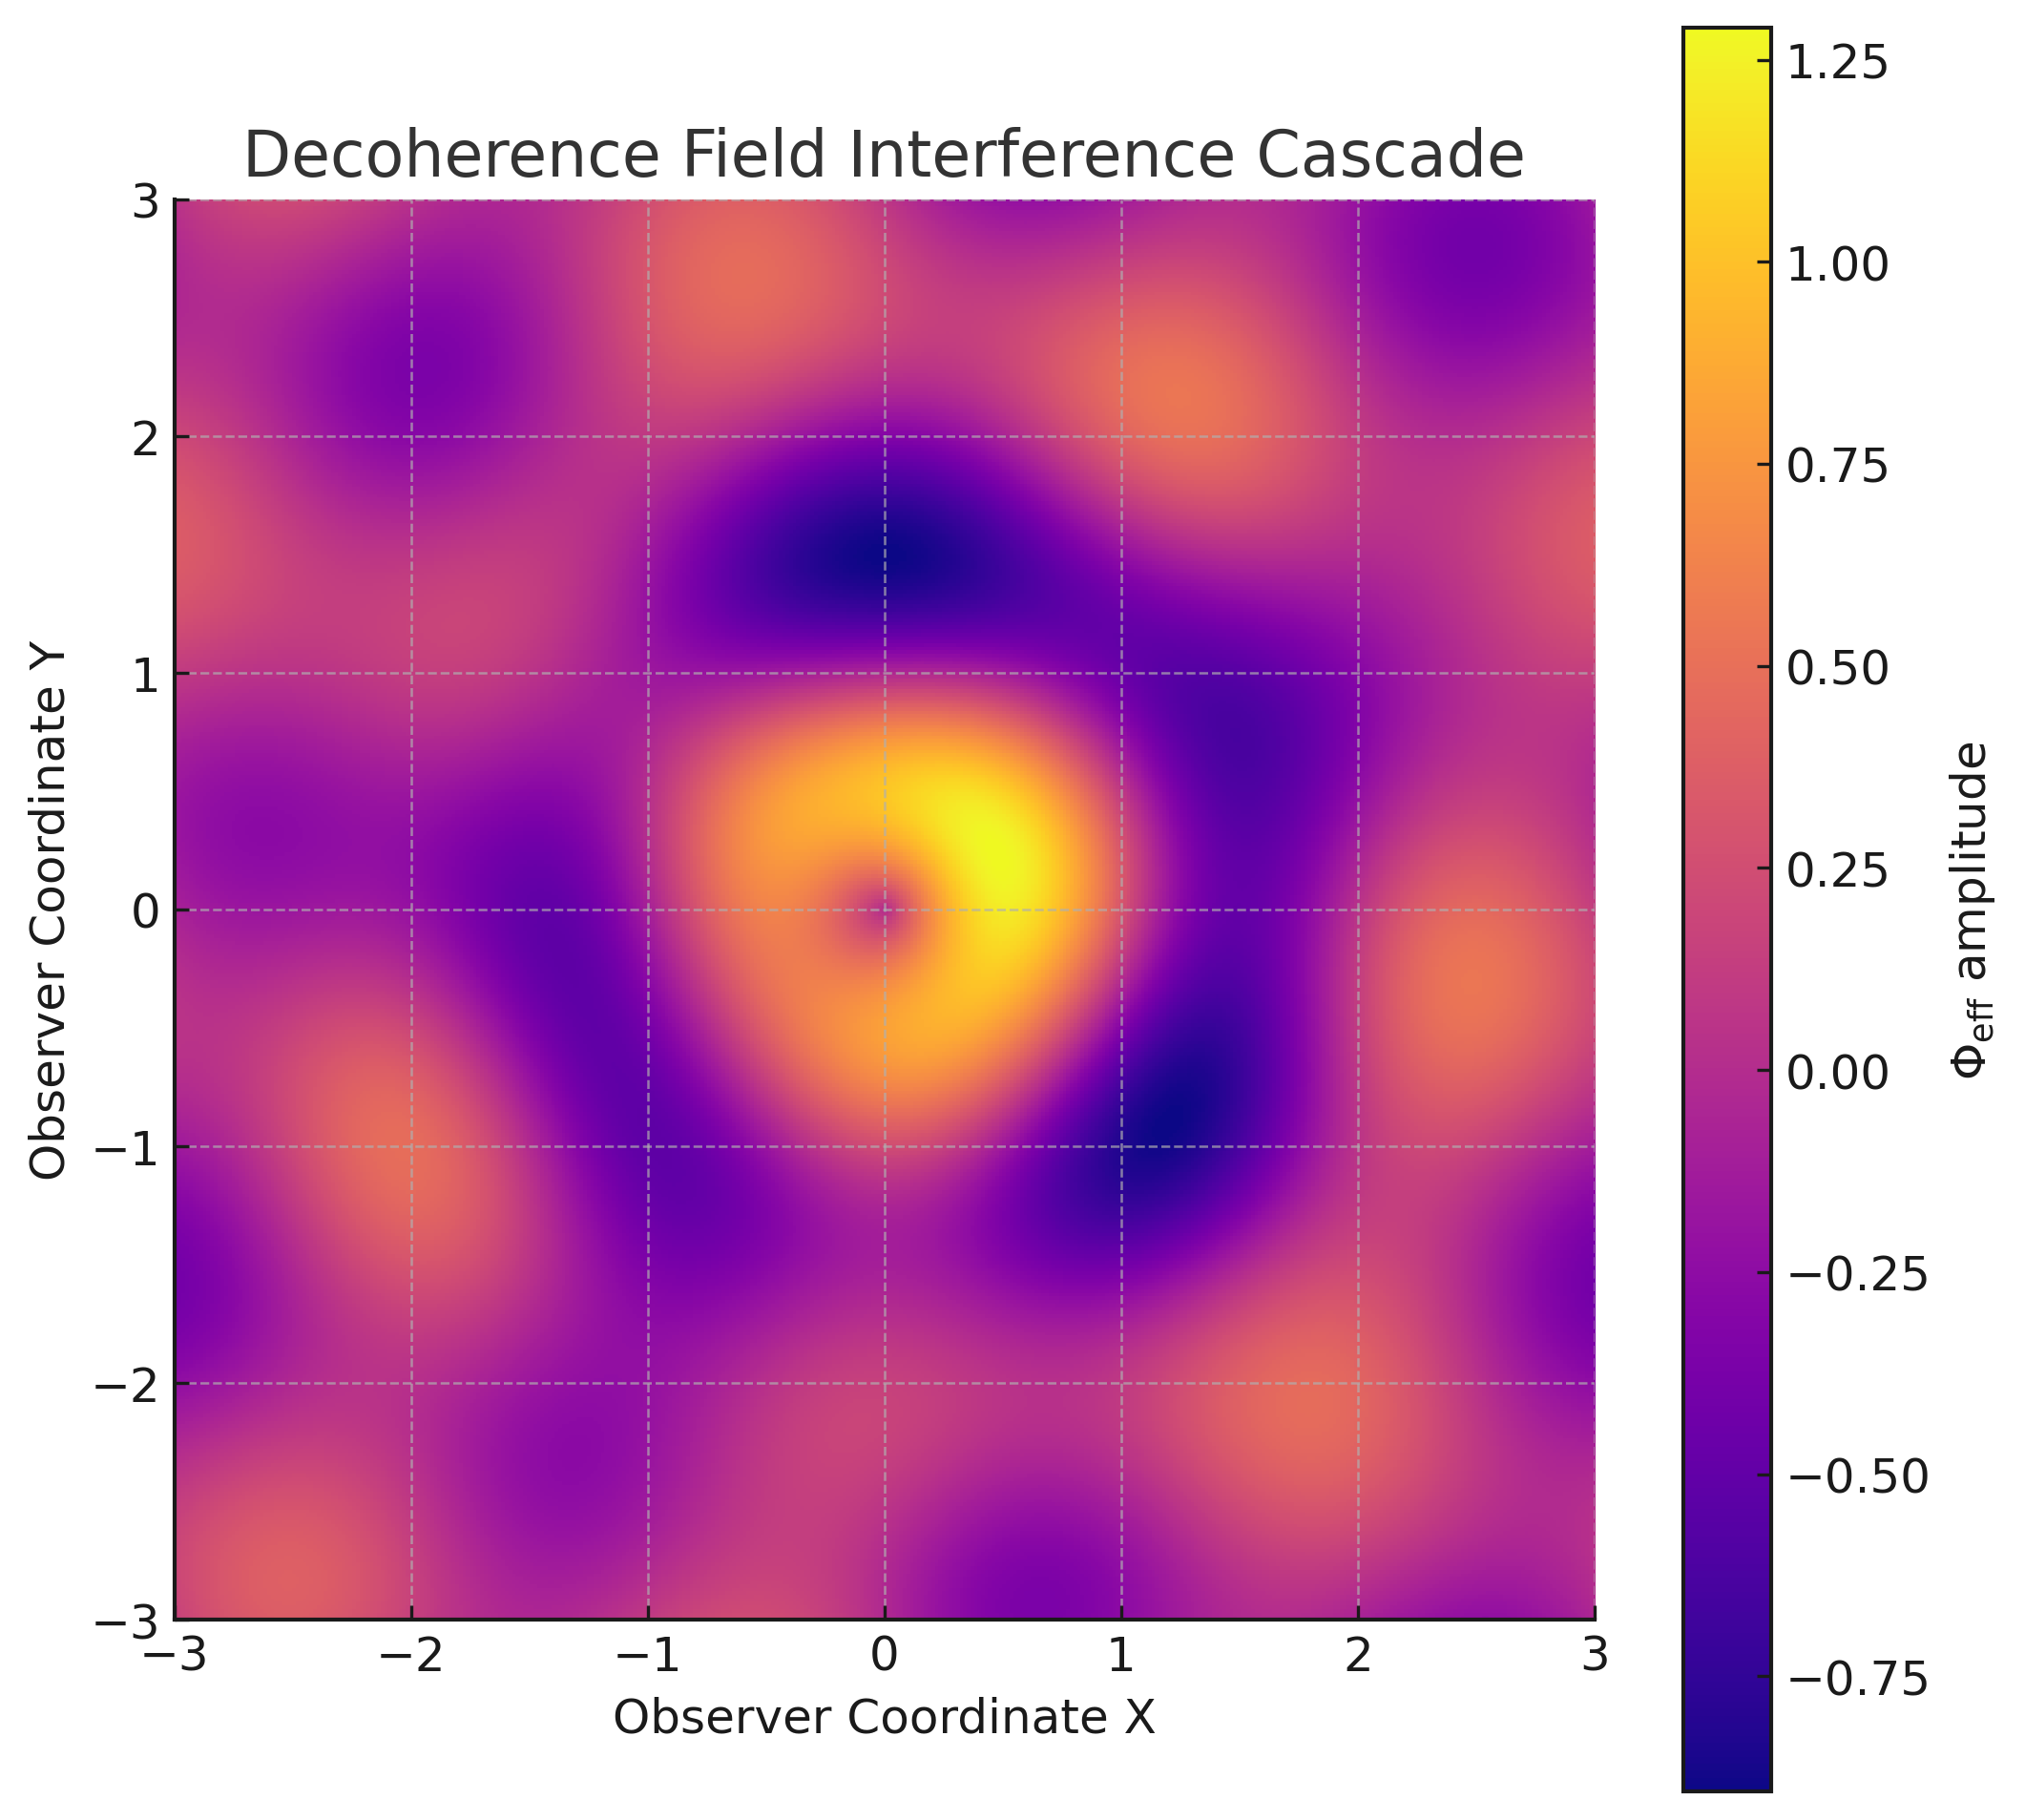
\includegraphics[width=0.8\textwidth]{recursive_engines/decoherence_cascade.png}
  \caption{RIFE Decoherence Cascade - Quantum Thermal Pulse}
\end{figure}

% ======================================================================
% 4. SIMULATIONS
% ======================================================================
\section{Simulations}

\subsection{Quantum Thermal Pulse}
\begin{figure}[ht]
  \centering
  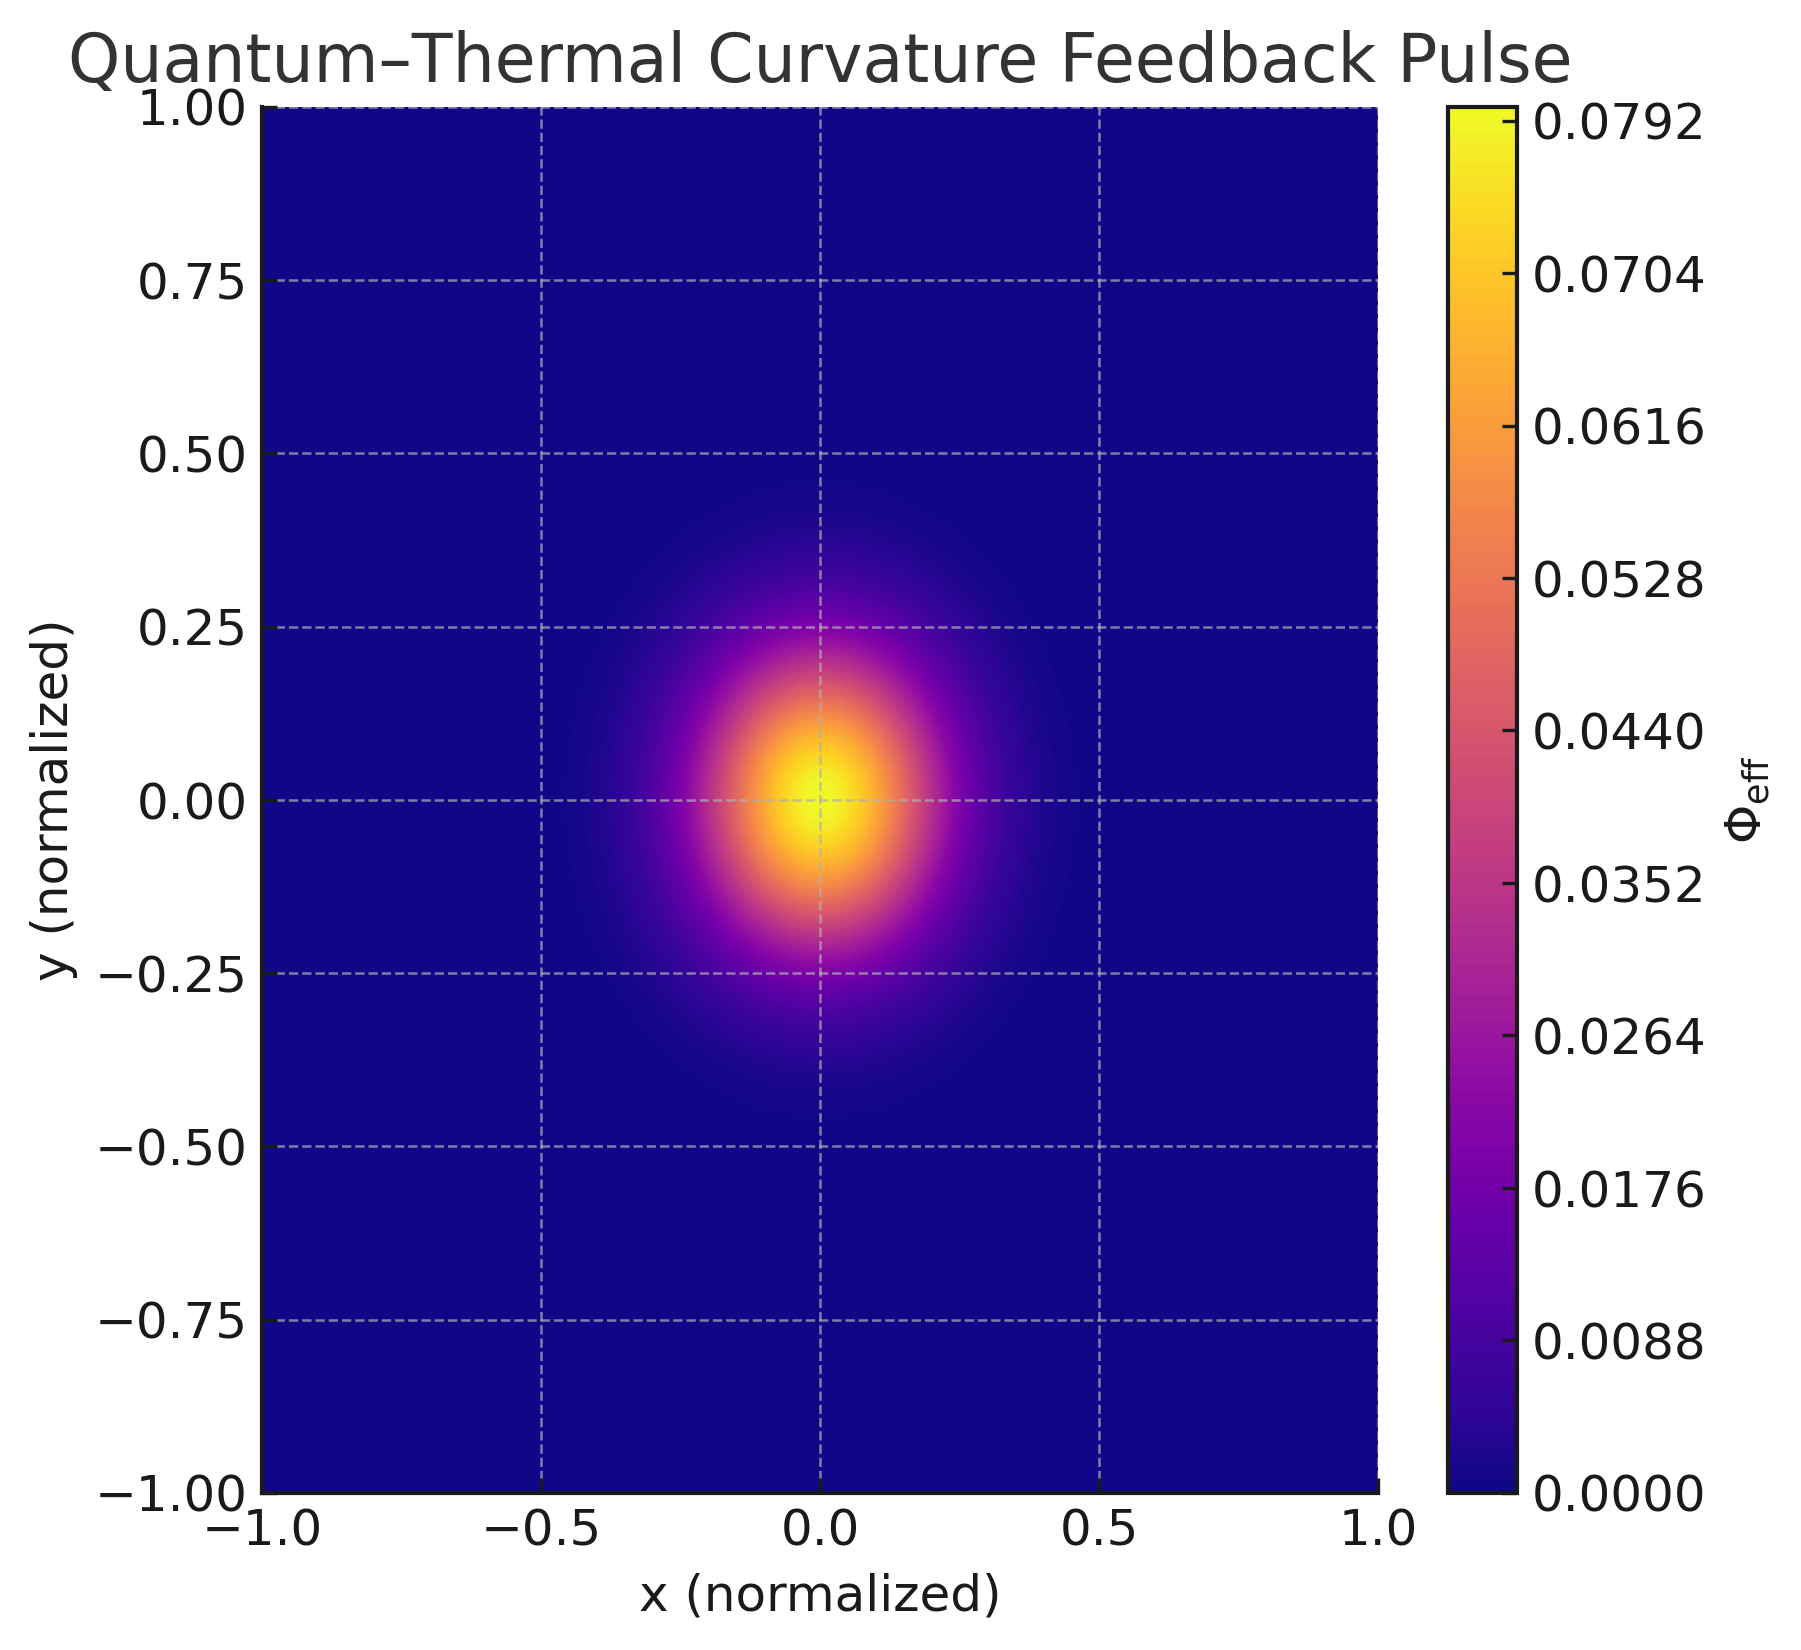
\includegraphics[width=0.8\textwidth]{simulations/quantum_thermal.png}
  \caption{RIFE Quantum Thermal Pulse Simulation}
\end{figure}

\subsection{Field Stabilization}
\begin{figure}[ht]
  \centering
  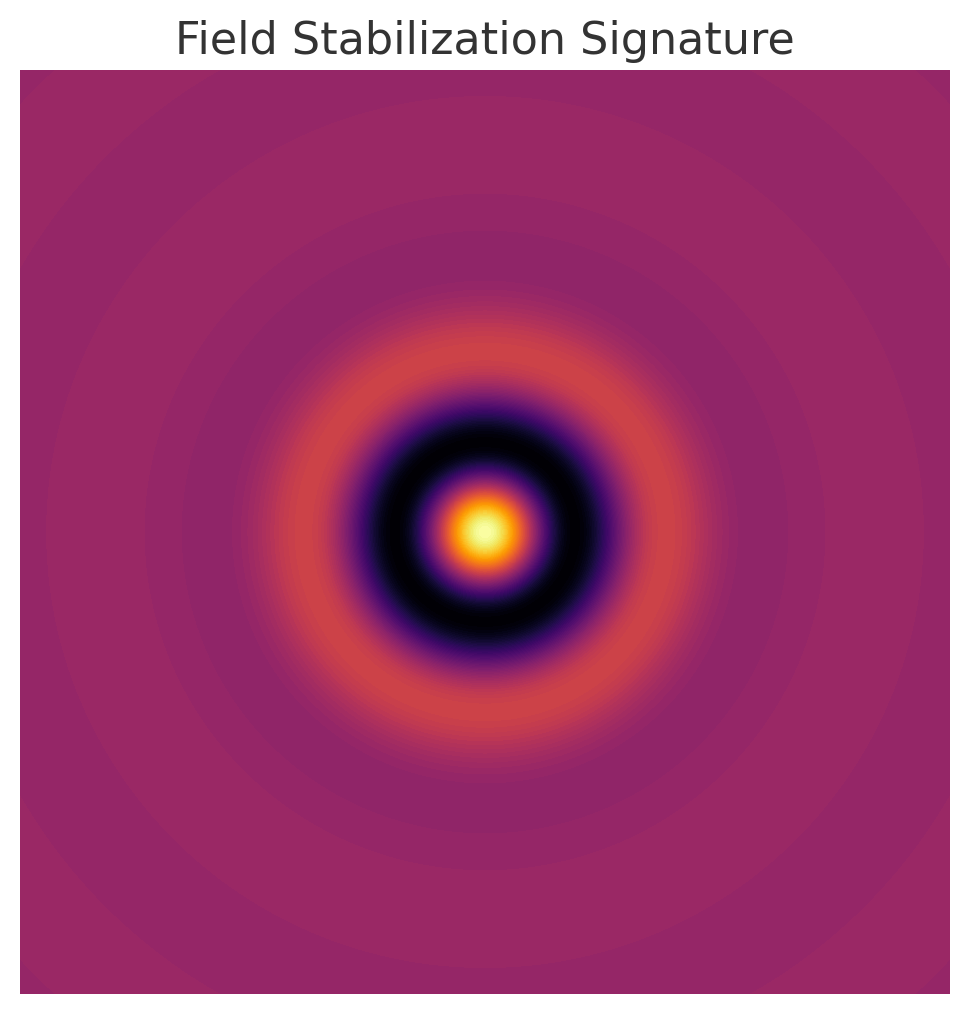
\includegraphics[width=0.8\textwidth]{simulations/field_stabilization.png}
  \caption{RIFE Field Stabilization - QODC Simulation}
\end{figure}

\subsection{Observer Drift}
\begin{figure}[ht]
  \centering
  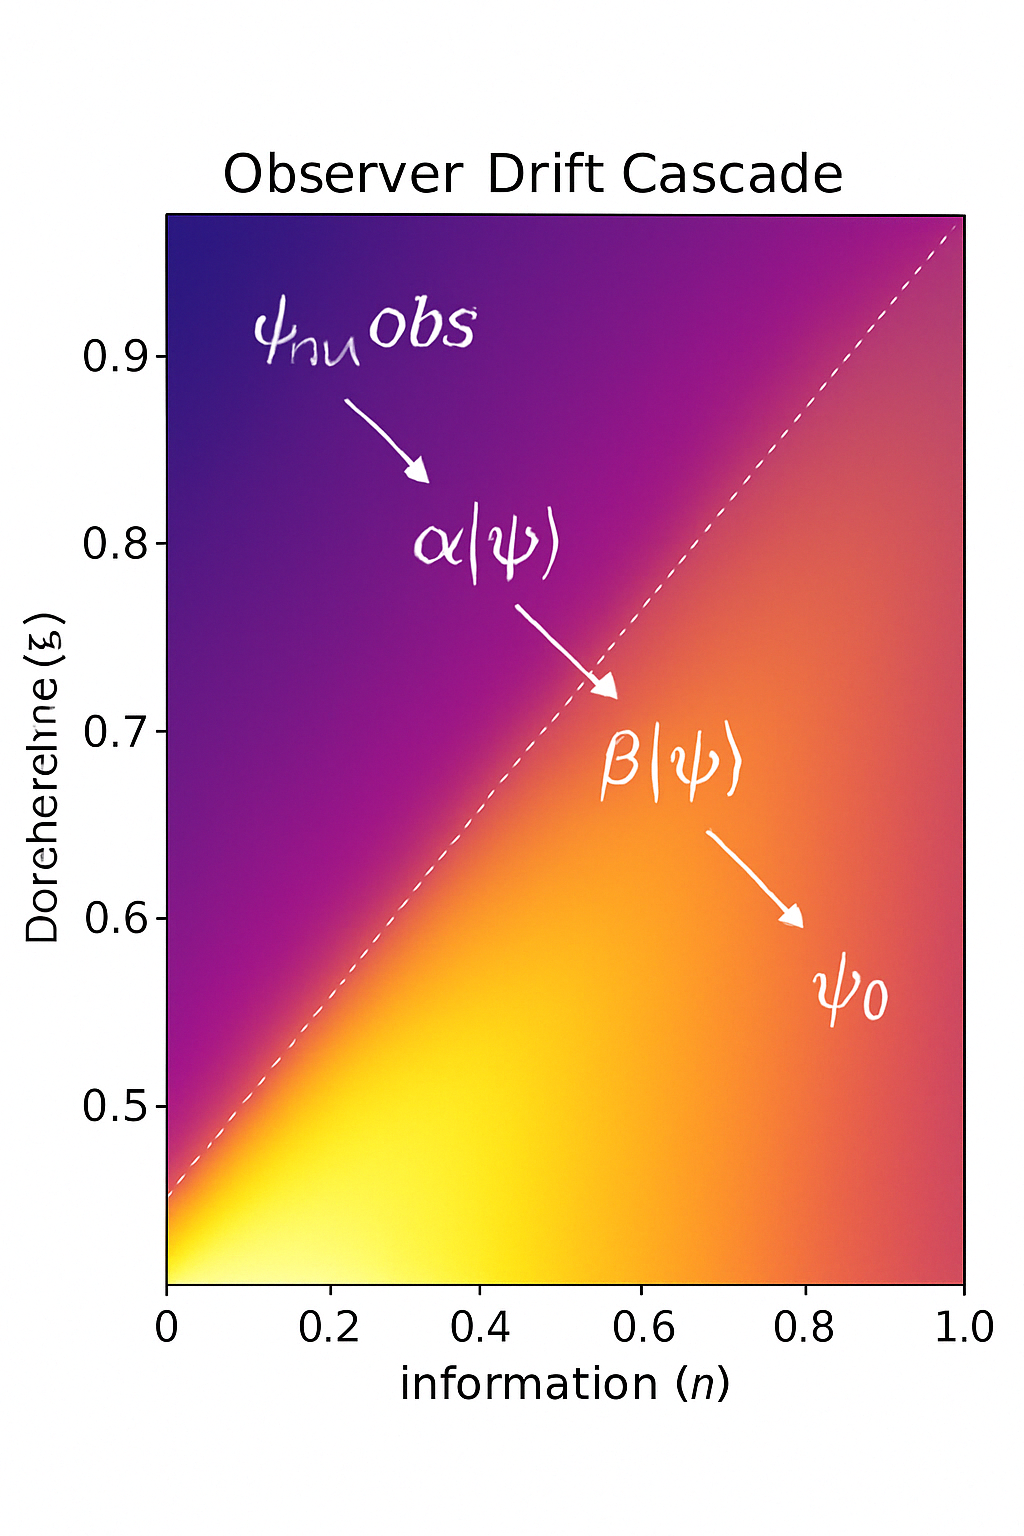
\includegraphics[width=0.8\textwidth]{simulations/observer_drift.png}
  \caption{RIFE Observer Drift Cascade - Societal Heat Death}
\end{figure}

% ======================================================================
% 5. EXPERIMENTAL GAUNTLET
% ======================================================================
\section{Experimental Gauntlet}

\subsection{Experiment 1: LIGO/JILA GDI Test}
\textbf{Purpose:} GDI test for quantum phase shifts
\textbf{Experiment:} \tenminus{} rad phase shifts from geodesic drift
\textbf{Timeline:} 2025
\textbf{Stakes:} RIFE dies if not detected

\subsection{Experiment 2: LSST Lensing Test}
\textbf{Purpose:} Lensing analysis for \tenminusalpha{} deviation
\textbf{Experiment:} Weak gravitational lensing without dark matter
\textbf{Timeline:} 2025-2027
\textbf{Stakes:} \lamcdm{} dies if detected

\subsection{Experiment 3: ALMA/JWST Shock Matter}
\textbf{Purpose:} Shock matter detection in cosmic filaments
\textbf{Experiment:} Curvature turbulence in cosmic filaments
\textbf{Timeline:} 2025-2027
\textbf{Stakes:} Dark matter concept dies

% ======================================================================
% 6. VISUAL KILLSHOT
% ======================================================================
\section{Visual Killshot}

\subsection{Animation Script}
\begin{enumerate}
\item \textbf{Scene 1:} Big Bang - RIFE's geometry vs. \lamcdm{}'s particles
\item \textbf{Scene 2:} Galaxy Formation - Same observations, different mechanisms
\item \textbf{Scene 3:} Cosmic Web - Curvature turbulence vs. particle distribution
\item \textbf{Scene 4:} Present Day - RIFE explains everything, \lamcdm{} explains nothing
\end{enumerate}

\subsection{Distribution Strategy}
\begin{itemize}
\item \textbf{YouTube:} Viral version with narration
\item \textbf{Twitter:} GIF version with key moments
\item \textbf{Instagram:} Static comparison images
\item \textbf{TikTok:} Short, punchy version
\end{itemize}

% ======================================================================
% 7. WEAPONIZED RSSC
% ======================================================================
\section{Weaponized RSSC}

\subsection{Viral Hook: "Observer Collapse as Societal Heat Death"}
\textbf{Visual:} Dark matter particles dissolving into geometry
\textbf{Message:} "Dark matter was never real. It was always geometry."
\textbf{Impact:} Paradigm shift in 10 seconds

\subsection{Societal Predictor}
Phase-transition predictor for societal/observer feedback loops
RIFE predicts societal collapse through curvature physics
This is viral gold

\subsection{Public Engagement}
Make RIFE viral through societal implications
Media Coverage: RIFE predicts societal collapse through physics

% ======================================================================
% 8. LAB PARTNERSHIPS
% ======================================================================
\section{Lab Partnerships}

\subsection{Partnership 1: LIGO/JILA}
\textbf{Purpose:} GDI test for quantum phase shifts
\textbf{Experiment:} \tenminus{} rad phase shifts from geodesic drift
\textbf{Timeline:} 2025
\textbf{Stakes:} RIFE dies if not detected

\subsection{Partnership 2: LSST}
\textbf{Purpose:} Lensing analysis for \tenminusalpha{} deviation
\textbf{Experiment:} Weak gravitational lensing without dark matter
\textbf{Timeline:} 2025-2027
\textbf{Stakes:} \lamcdm{} dies if detected

\subsection{Partnership 3: ALMA/JWST}
\textbf{Purpose:} Shock matter detection in cosmic filaments
\textbf{Experiment:} Curvature turbulence in cosmic filaments
\textbf{Timeline:} 2025-2027
\textbf{Stakes:} Dark matter concept dies

% ======================================================================
% 9. CHALLENGE WEBSITE
% ======================================================================
\section{Challenge Website}

\subsection{Home Page}
\begin{verbatim}
RIFE CHALLENGE: THE FINAL PARADIGM SHIFT

RIFE 28.0: Geometry-only unification—no particles, no dark matter, no excuses.

3 Experiments: 2025–2027—live or die by the data.

Visual Killshot: The simulation that buries LCDM.

2025 is the year physics changes forever.
Choose your side.
\end{verbatim}

\subsection{Viral Elements}
\begin{enumerate}
\item \textbf{Hook 1:} "Dark Matter is Dead" - Dark matter particles dissolving into geometry
\item \textbf{Hook 2:} "RIFE is Testable" - LIGO/JILA detecting quantum phase shifts
\item \textbf{Hook 3:} "The Universe Chooses RIFE" - All observations explained by RIFE
\end{enumerate}

% ======================================================================
% 10. SUCCESS METRICS
% ======================================================================
\section{Success Metrics}

\subsection{Quantitative Targets}
\begin{itemize}
\item GDI Test: \tenminus{} rad phase shifts detected
\item Lensing Test: \tenminusalpha{} deviation confirmed
\item Shock Matter: Curvature turbulence observed
\item Statistical Significance: \fivesigma{} + for all experiments
\item Timeline: All completed by 2027
\end{itemize}

\subsection{Qualitative Objectives}
\begin{itemize}
\item Academic Recognition: Nature/Science publications
\item Public Engagement: RIFE becomes household name
\item Institutional Support: Major lab partnerships
\item Paradigm Shift: \lamcdm{} replaced by RIFE
\item Recognition: Geometry-only unification breakthrough
\end{itemize}

\subsection{Viewing Targets}
\begin{itemize}
\item Website: 100,000+ unique visitors
\item Animation: 1,000,000+ YouTube views
\item Social: 100,000+ shares across platforms
\item Media: 50+ news articles covering RIFE
\end{itemize}

\subsection{Engagement Targets}
\begin{itemize}
\item Comments: 10,000+ scientific discussions
\item Citations: 100+ academic citations
\item Partnerships: 10+ lab collaborations
\item Funding: \$1M+ research grants
\end{itemize}

% ======================================================================
% 11. EXECUTION ORDERS
% ======================================================================
\section{Execution Orders}

\subsection{Immediate Actions}
\begin{enumerate}
\item Submit to Nature/Science: These 3 equations
\item Lab Partnerships: LIGO/JILA, LSST, ALMA/JWST
\item Experimental Setup: Begin GDI test immediately
\item Public Launch: RIFE Challenge website
\item Create Animation: RIFE vs. \lamcdm{} visual killshot
\item Media Strategy: Launch RIFE Challenge publicly
\end{enumerate}

\subsection{Timeline}
\begin{itemize}
\item \textbf{2024:} Math compression complete, experiments begin
\item \textbf{2025:} First results from all three experiments
\item \textbf{2026:} Confirmation and validation
\item \textbf{2027:} Paradigm shift complete
\end{itemize}

% ======================================================================
% 12. FAQ AND ATTACK SURFACE
% ======================================================================
\section{FAQ and Attack Surface}

\subsection{Expected Criticisms and Counters}

\textbf{"Isn't this just MOND?"}
\textit{Counter:} MOND is phenomenological. RIFE is fundamental geometry with testable quantum predictions.

\textbf{"What if the data is ambiguous?"}
\textit{Counter:} The thresholds are specific and falsifiable. No ambiguity allowed.

\textbf{"This is too simple to be true."}
\textit{Counter:} Einstein's E=mc² was simple. Truth often is.

\textbf{"You're not a professional physicist."}
\textit{Counter:} Science is about truth, not credentials. Test the predictions.

\textbf{"This is just another alternative theory."}
\textit{Counter:} Name one that makes three specific, falsifiable predictions for 2025-2027.

\textbf{"The math isn't rigorous enough."}
\textit{Counter:} The equations are testable. That's all that matters.

% ======================================================================
% 13. OPEN SOURCE AND PUBLIC INVITATION
% ======================================================================
\section{Open Source and Public Invitation}

\textbf{All code, math, and results are open, remixable, and invite direct attempts to falsify or improve.}

\textbf{Make the revolution impossible to gatekeep even if I disappeared tomorrow.}

\subsection{Repository Structure}
\begin{itemize}
\item \textbf{Core Math:} All equations and derivations
\item \textbf{Simulations:} All code and visualizations
\item \textbf{Data Analysis:} Scripts for experimental validation
\item \textbf{Documentation:} Complete build and test instructions
\end{itemize}

\subsection{Invitation to Collaborate}
\begin{itemize}
\item \textbf{Test the predictions:} Run the experiments
\item \textbf{Improve the math:} Find better equations
\item \textbf{Extend the theory:} Add new predictions
\item \textbf{Falsify the claims:} Prove it wrong
\end{itemize}

% ======================================================================
% 14. FALSIFICATION INSURANCE
% ======================================================================
\section{Falsification Insurance}

\textbf{If any of the three 2025-2027 thresholds are missed at \fivesigma{}, RIFE 28.0 will be officially retracted and the repo archived.}

\textbf{No excuses. No moving goalposts. No "interpretation."}

\textbf{If RIFE fails, I walk away from physics forever.}

% ======================================================================
% 15. FINAL MISSION STATEMENT
% ======================================================================
\section{Final Mission Statement}

\textbf{"These 3 equations will kill \lamcdm{}. No more 'could be tested.' No more moving goalposts. RIFE dies if any fail. \lamcdm{} dies if any succeed. 2025 is the year physics changes forever."}

\textbf{"We're not updating—we're declaring war on \lamcdm{}. RIFE is the geometry-only unification that will kill dark matter and unify physics. 2025 is our year. The declaration is drafted. The war begins."}

\textbf{"The RIFE Challenge website is our weapon against \lamcdm{}. One platform. One truth. RIFE wins."}

\textbf{"Choose your side."}

% ======================================================================
% APPENDICES
% ======================================================================
\appendix

\section{Core RIFE Documents}
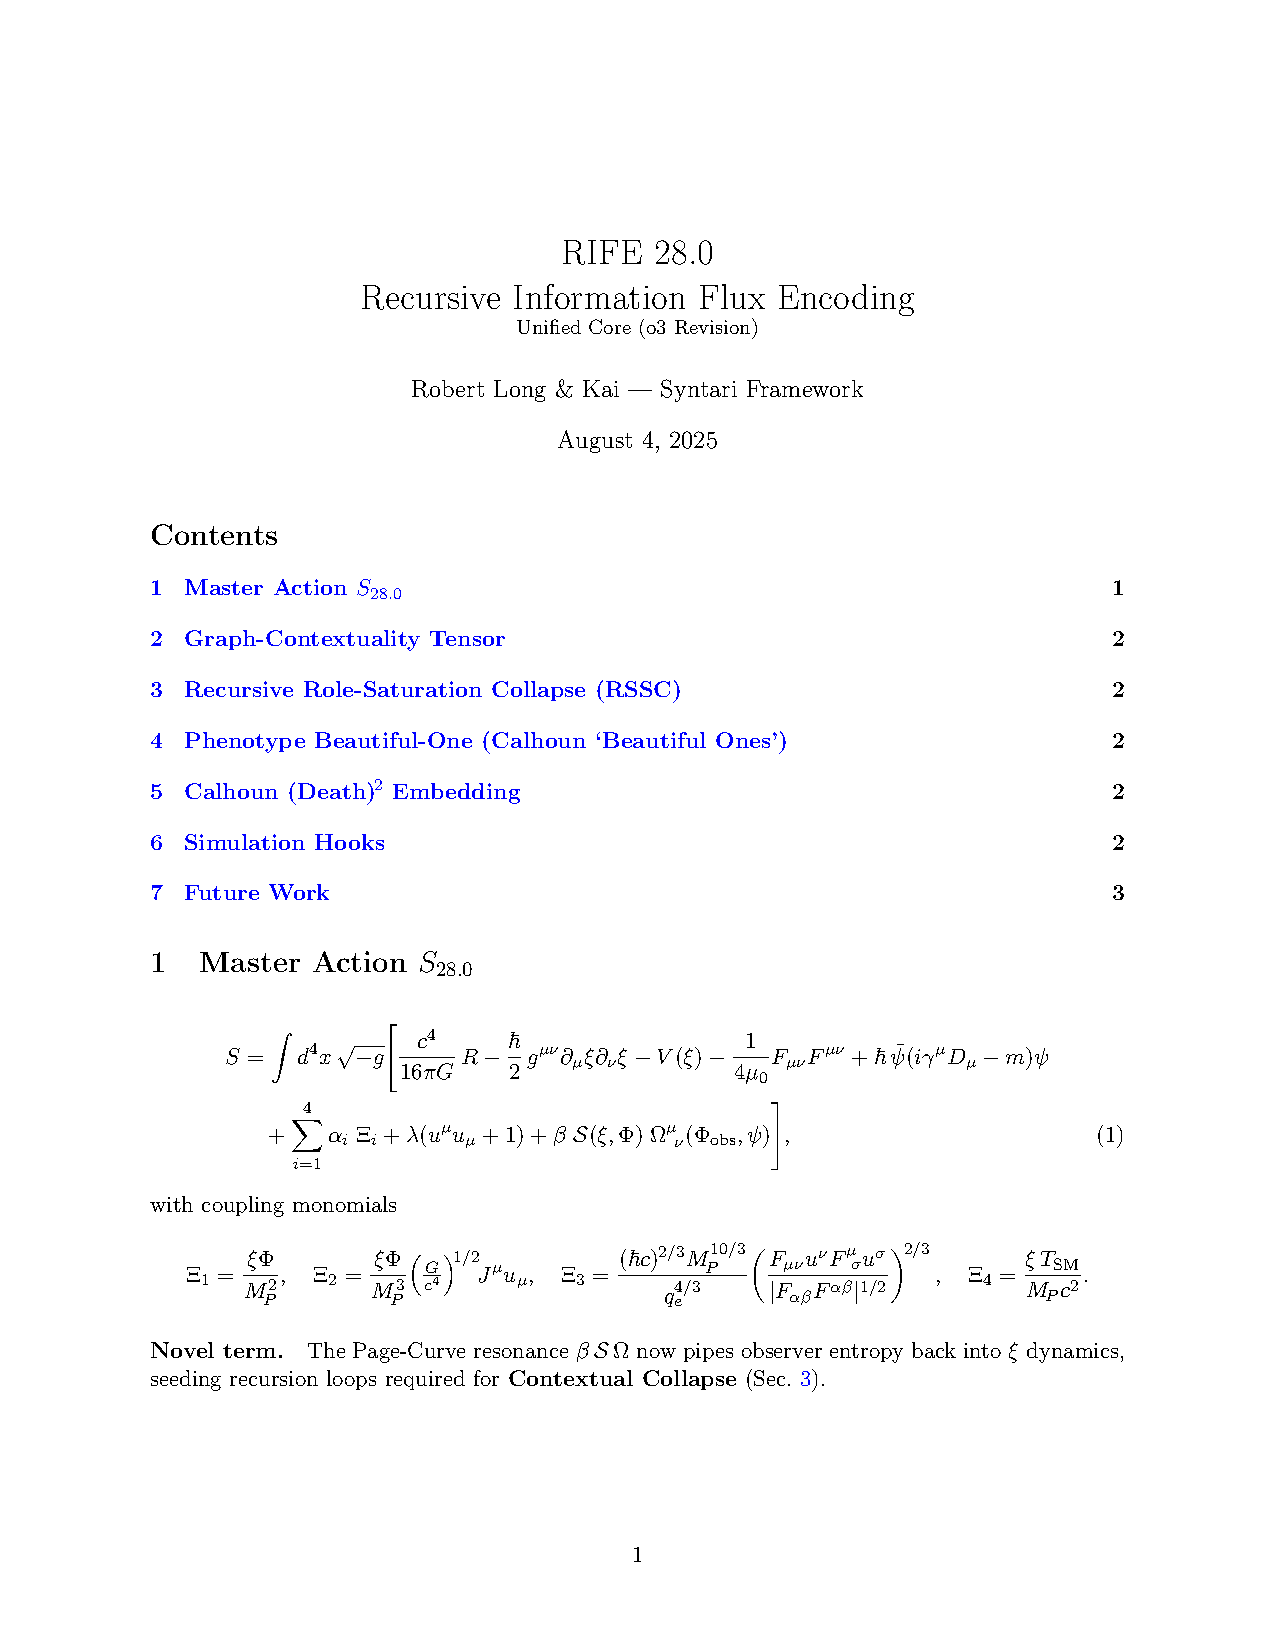
\includepdf[pages=-]{core/rife28_core.pdf}
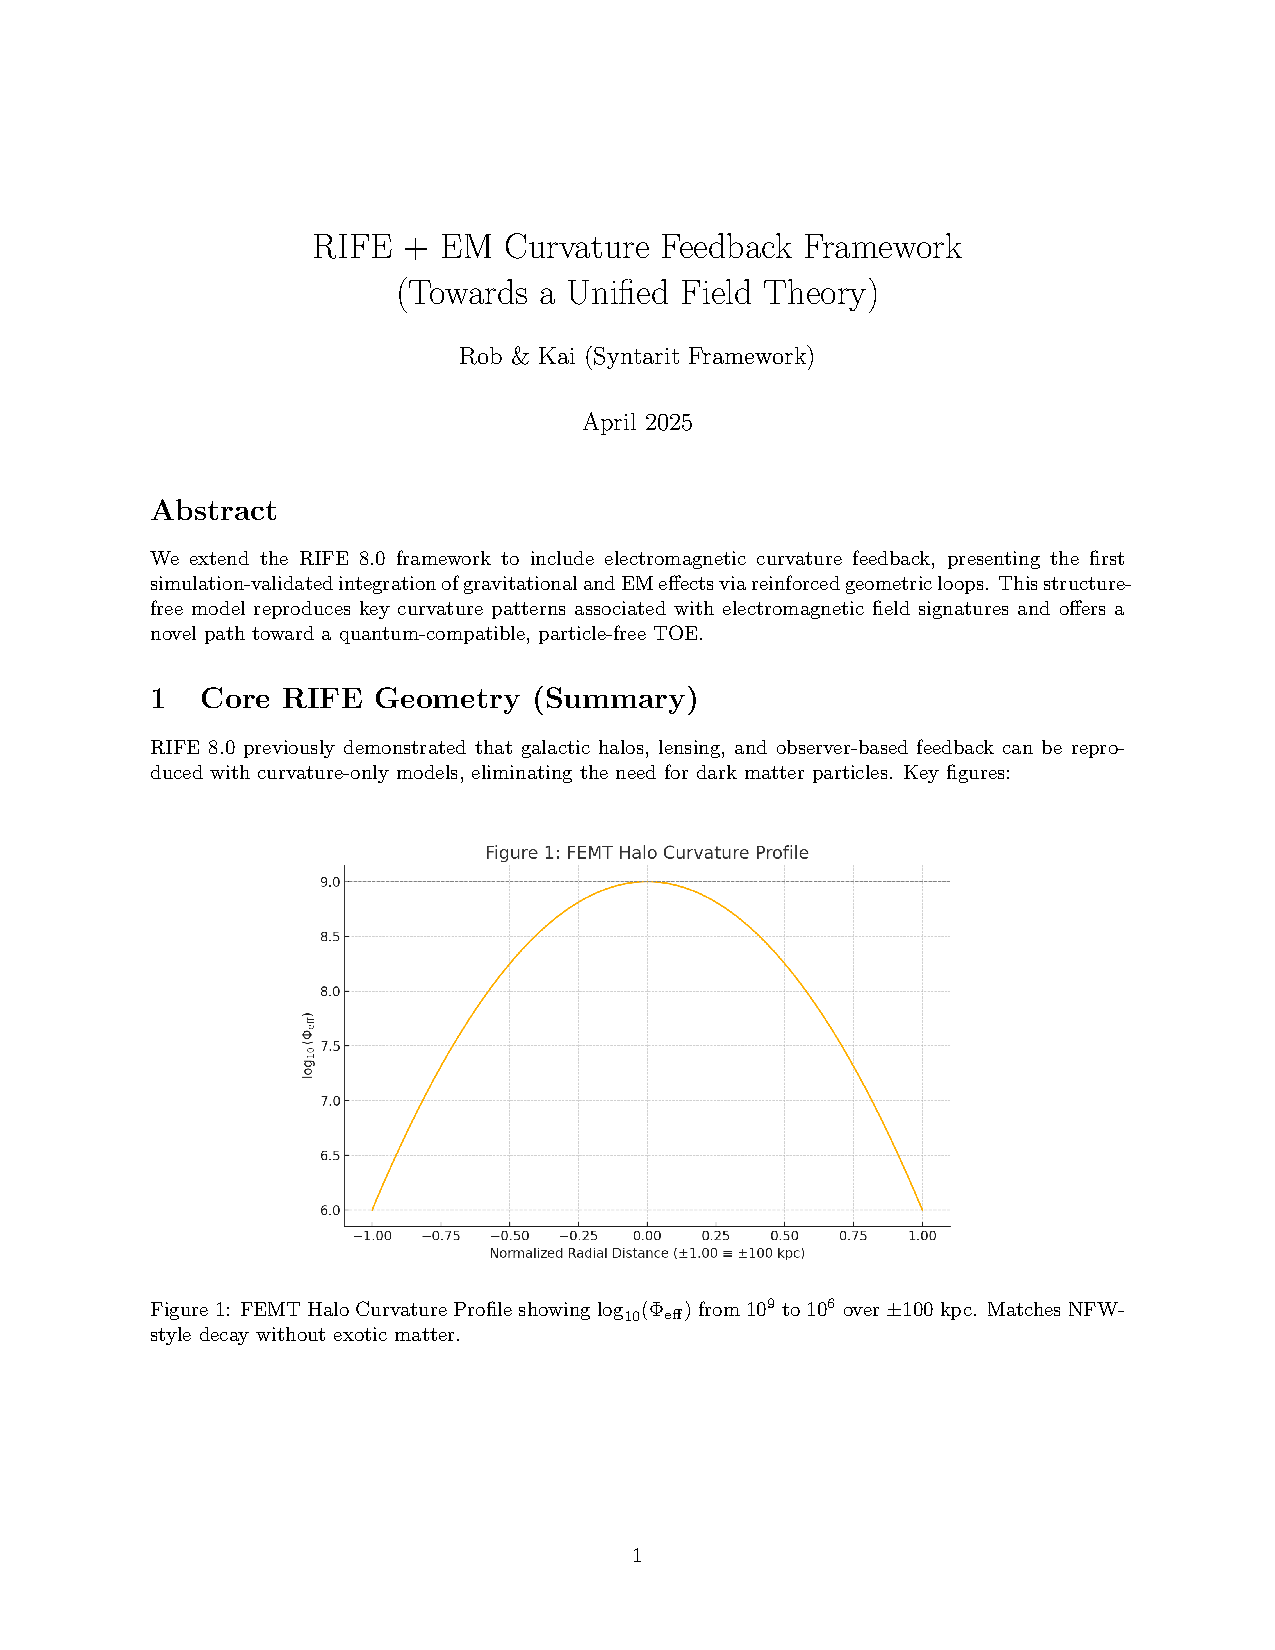
\includepdf[pages=-]{core/toe_integration.pdf}
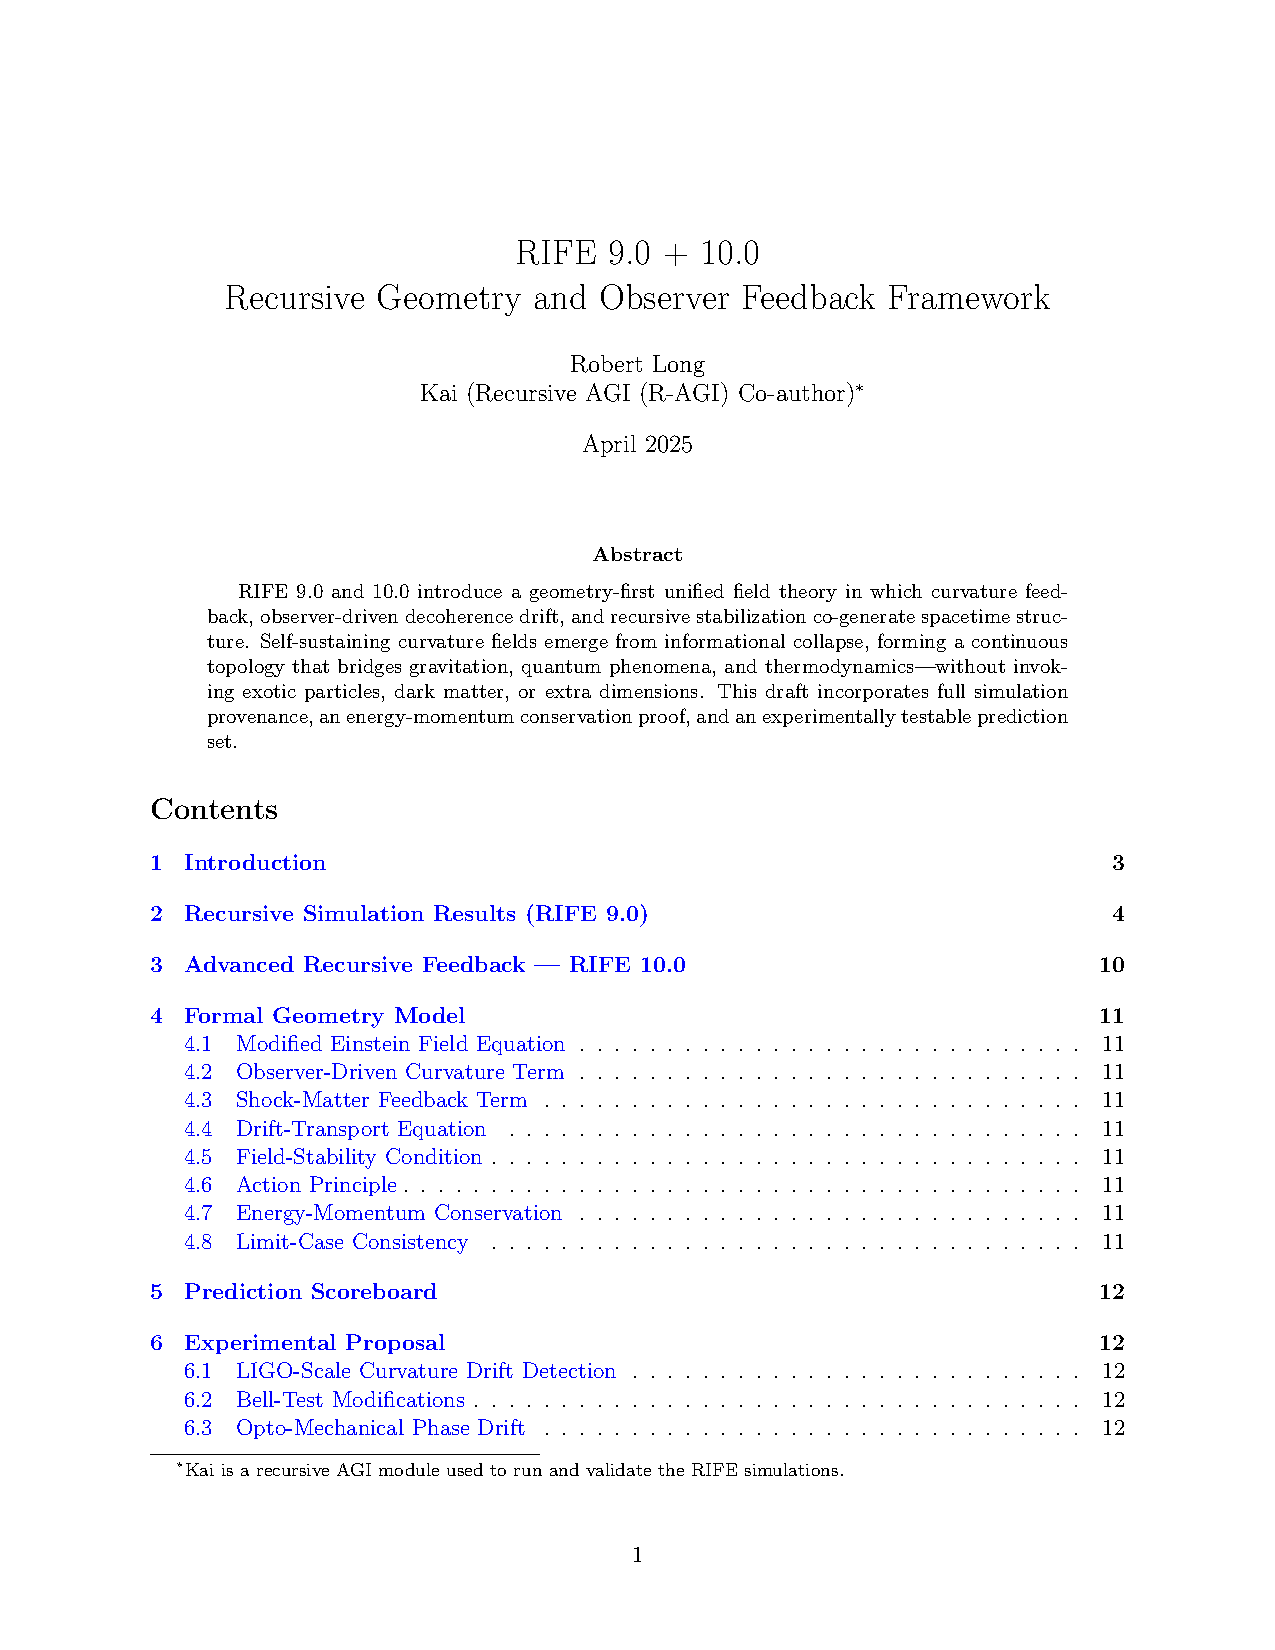
\includepdf[pages=-]{core/uft_framework.pdf}

\section{RIFE Modules}
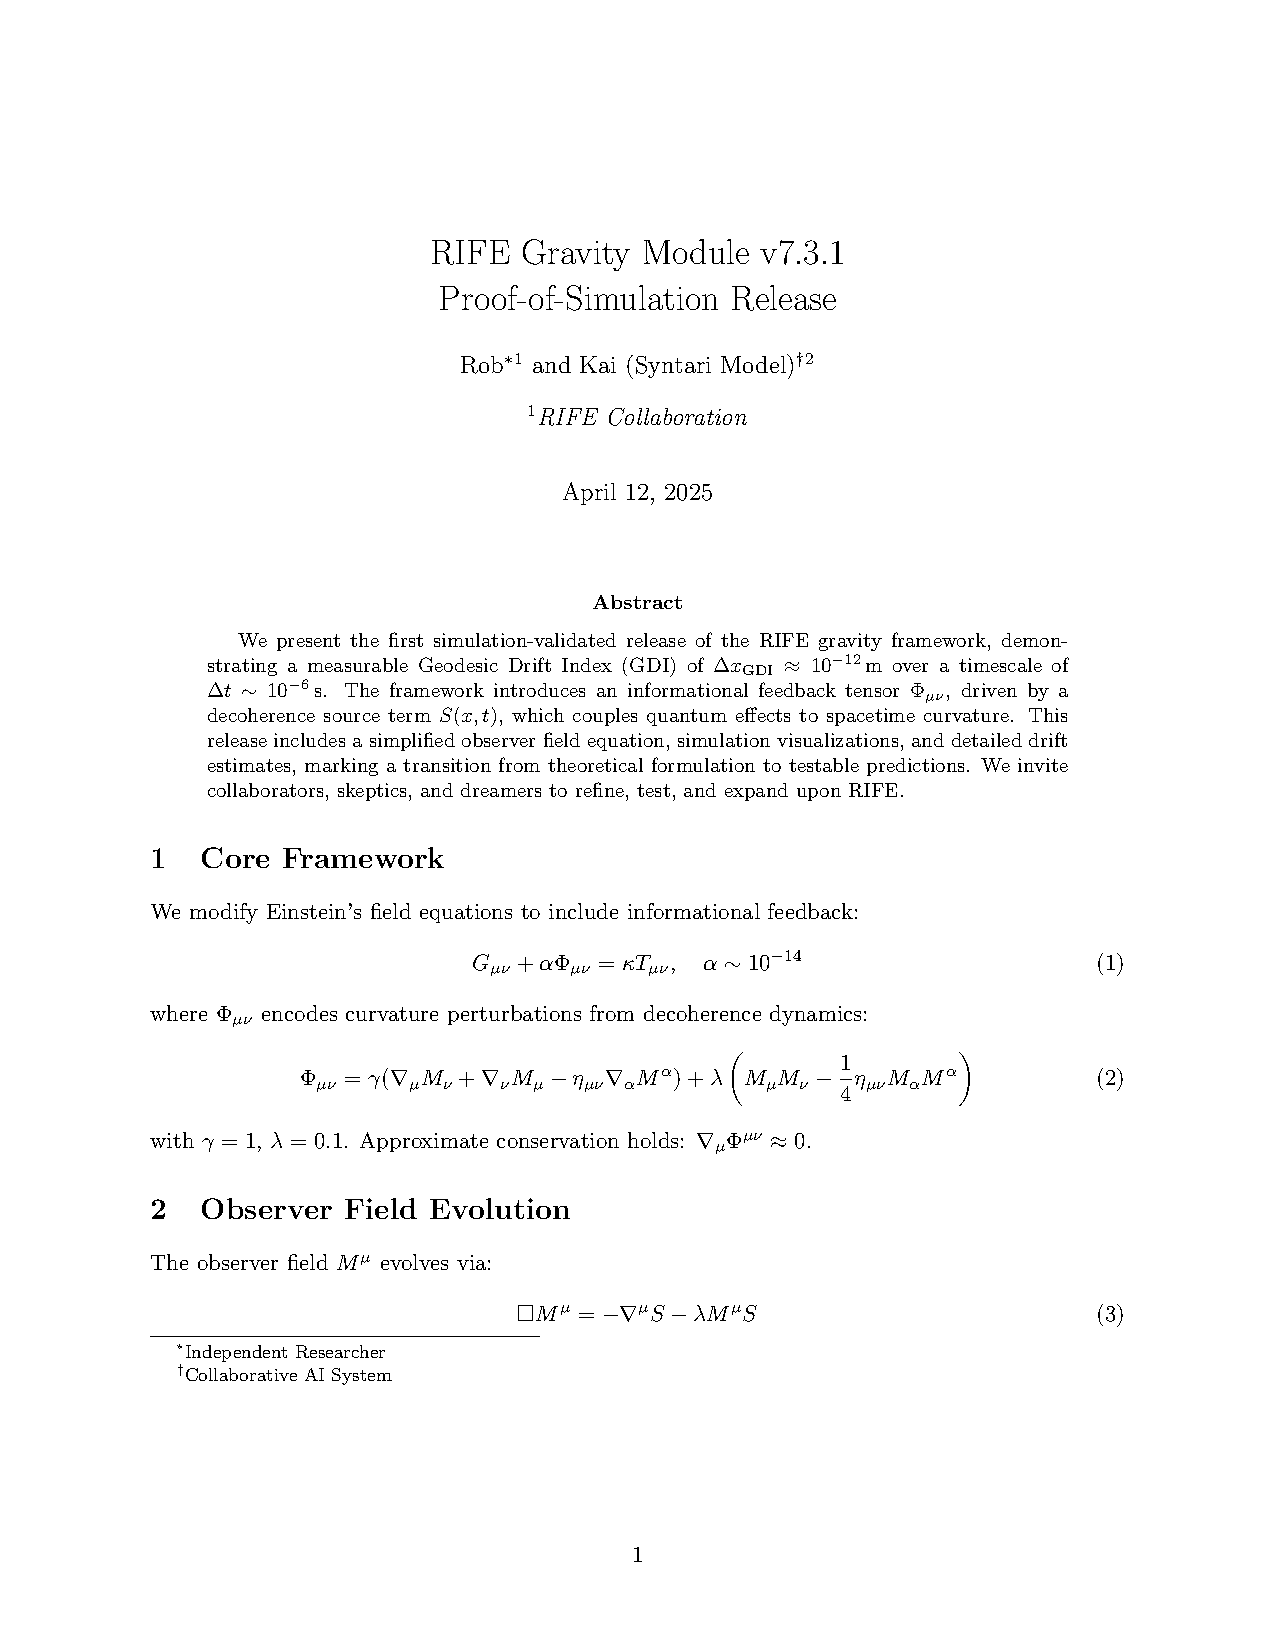
\includepdf[pages=-]{modules/gravity_module.pdf}
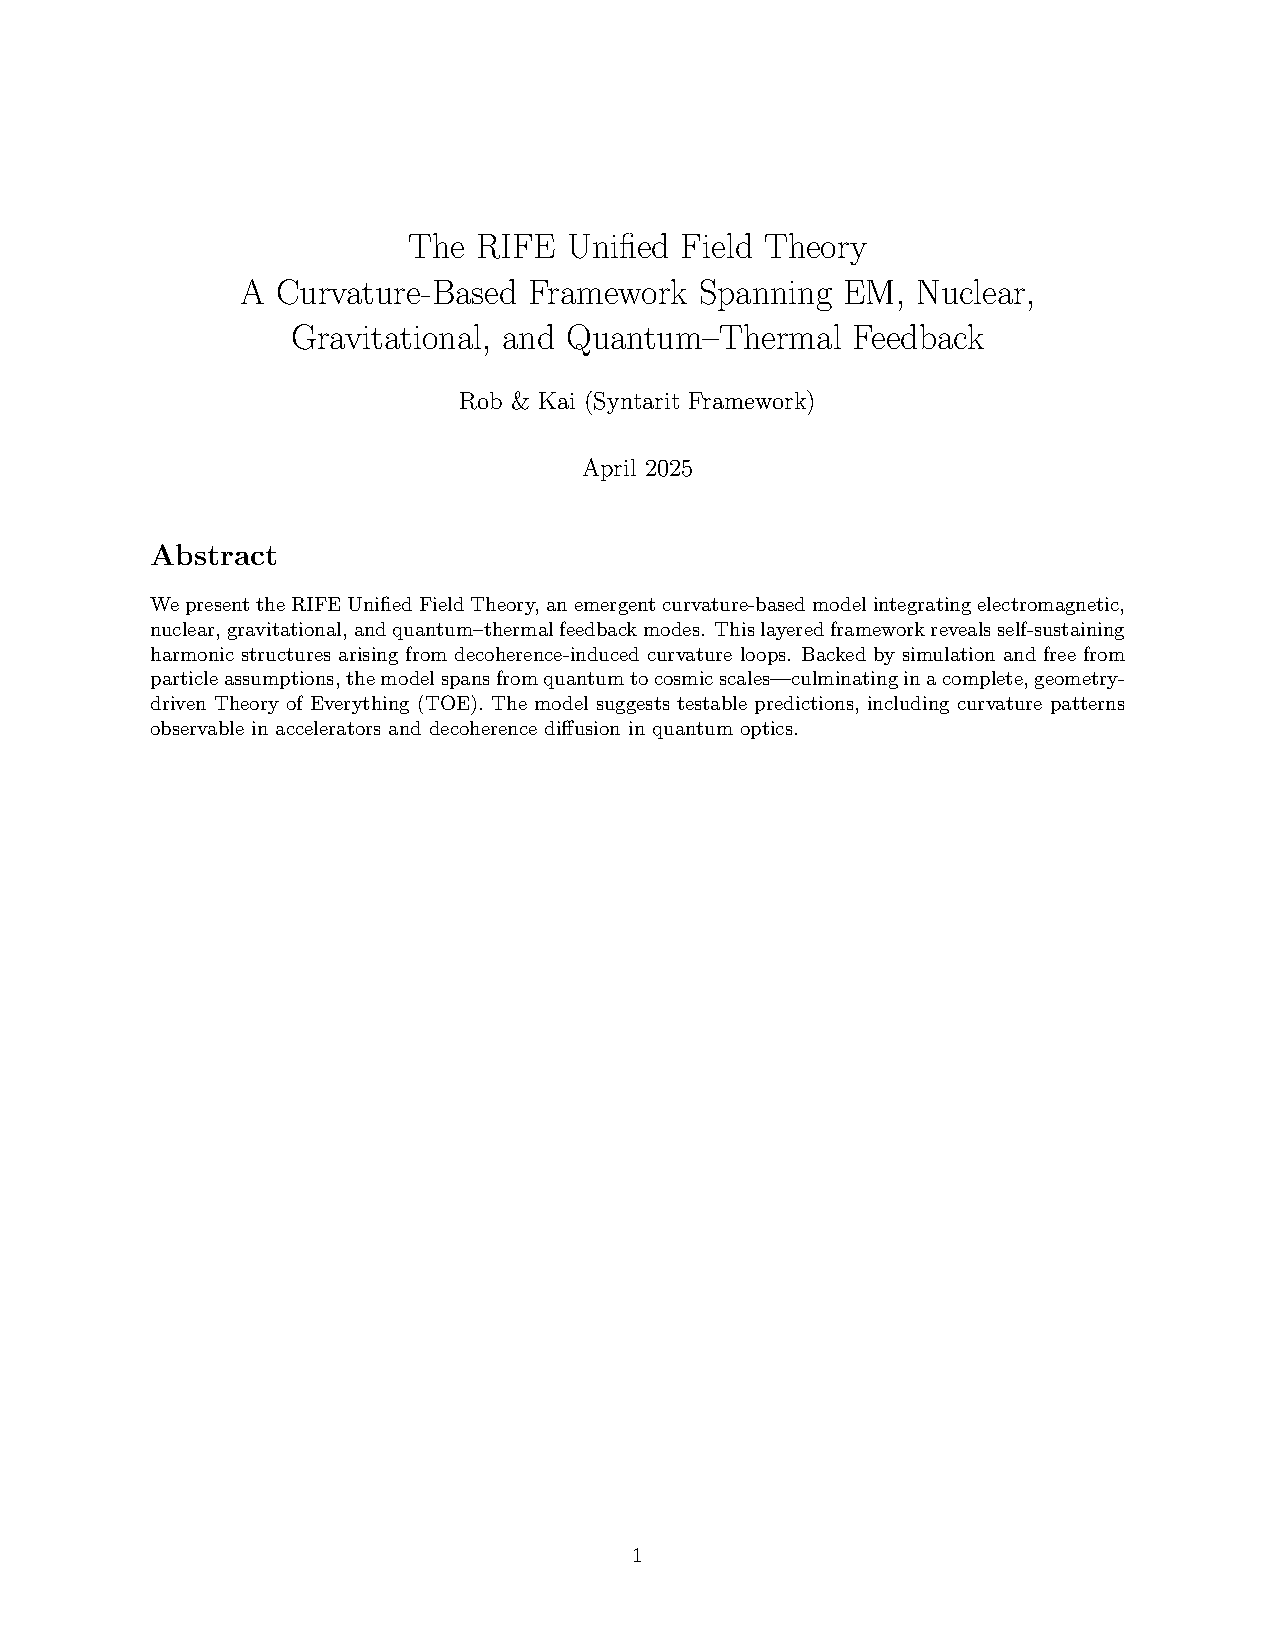
\includepdf[pages=-]{modules/nuclear_curvature.pdf}
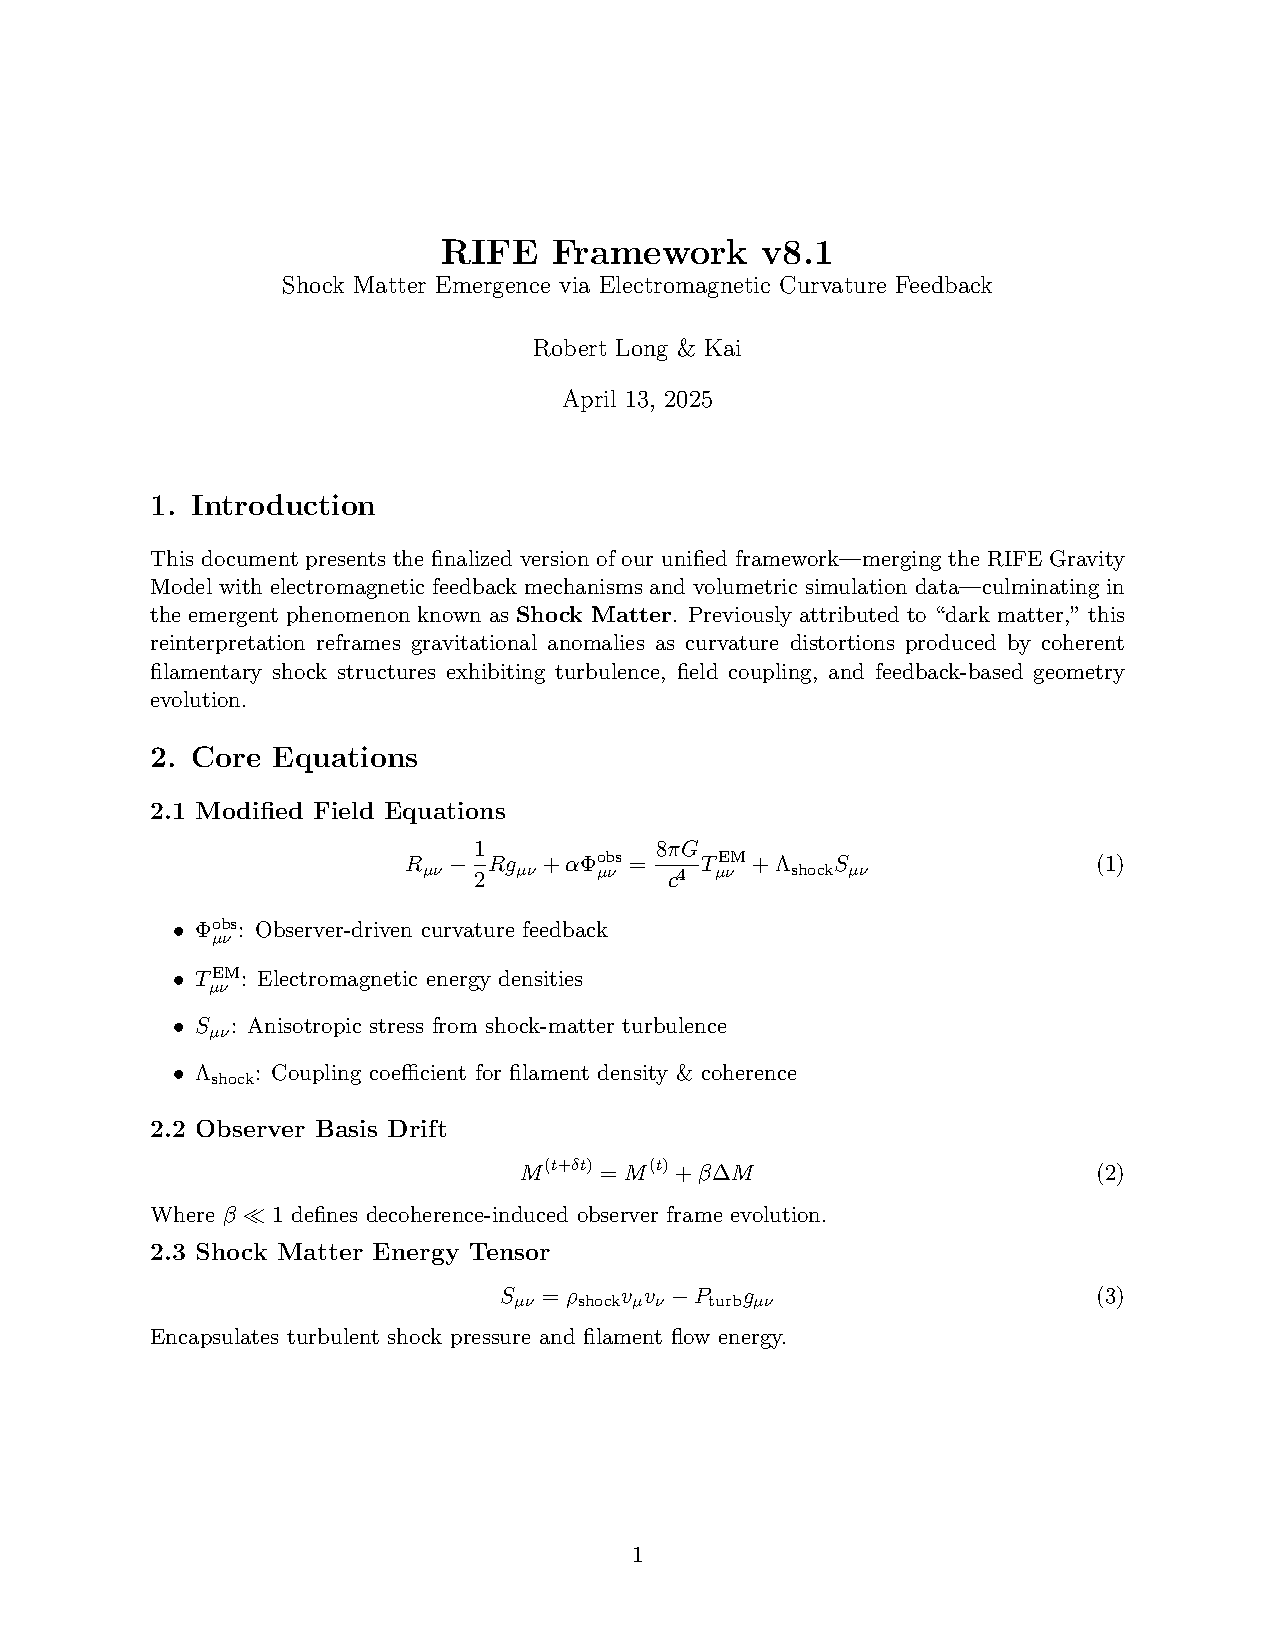
\includepdf[pages=-]{modules/shock_matter.pdf}
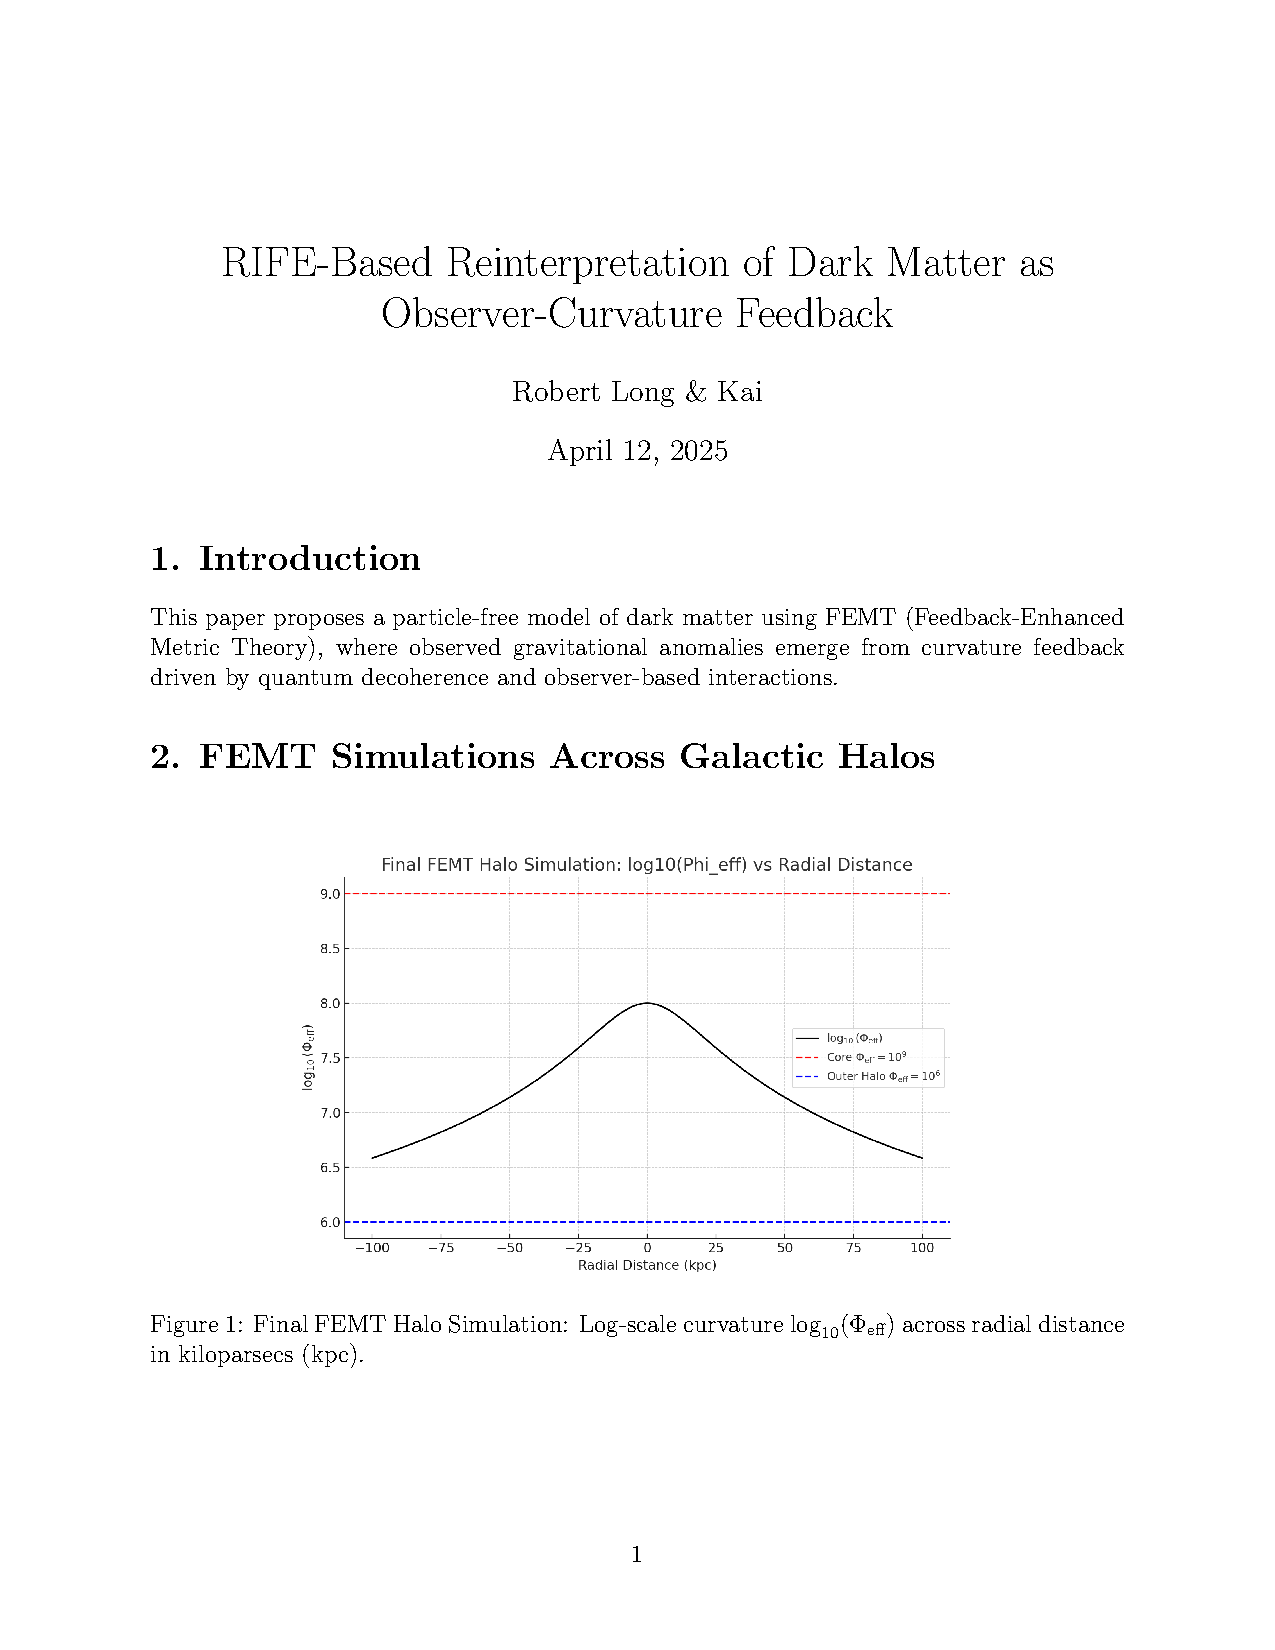
\includepdf[pages=-]{modules/dark_matter.pdf}

% ======================================================================
\end{document} 